\documentclass[a4paper,10pt]{article}
\usepackage[latin1]{inputenc}

\sloppy

%%%%%%%%%%%%%%%%%%%%%%%%%%%%%%%%%%%%%%%%%%%%%%%%%%%%%%%%%%%%
% PACKAGES
%%%%%%%%%%%%%%%%%%%%%%%%%%%%%%%%%%%%%%%%%%%%%%%%%%%%%%%%%%%%
\usepackage{amsmath, amssymb, url}
\usepackage[ruled,vlined]{algorithm2e}
% \usepackage[lined,boxed]{algorithm2e}

\newcommand{\LinesNumbered}{\linesnumbered}
\newcommand{\IncMargin}{\incmargin}
\newcommand{\DecMargin}{\decmargin}

\LinesNumbered


%%%%%%%%%%%%%%%%%%%%%%%%%%%%%%%%%%%%%%%%%%%%%%%%%%%%%%%%%%%%
% TIKZ
%%%%%%%%%%%%%%%%%%%%%%%%%%%%%%%%%%%%%%%%%%%%%%%%%%%%%%%%%%%%
\usepackage{pgf}
\usepackage{tikz}
\usetikzlibrary{arrows}
\usetikzlibrary{decorations.pathmorphing} 
% Couleurs
\definecolor{turquoise}{rgb}{0 0.41 0.41}
\definecolor{rouge}{rgb}{0.79 0.0 0.1}
\definecolor{vert}{rgb}{0.15 0.4 0.1}
\definecolor{mauve}{rgb}{0.6 0.4 0.8}
\definecolor{violet}{rgb}{0.58 0. 0.41}
\definecolor{orange}{rgb}{0.8 0.4 0.2}
\definecolor{bleu}{rgb}{0.39, 0.58, 0.93}
\definecolor{gris}{rgb}{0.6,0.6,0.6}
\definecolor{grisfonce}{rgb}{0.4,0.4,0.4}
% Jeu de couleurs pales
\definecolor{cpale1}{rgb}{1, 0.3, 0.3}
\definecolor{cpale2}{rgb}{0.3, 1, 0.3}
\definecolor{cpale3}{rgb}{0.3, 0.3, 1}
\definecolor{cpale4}{rgb}{1, 0.3, 1}
\definecolor{cpale5}{rgb}{1, 1, 0.3}
\definecolor{cpale6}{rgb}{0.3, 1, 1}
\definecolor{cpale7}{rgb}{0.9, 0.6, 0.2}
\definecolor{cpale8}{rgb}{0.7, 0.4, 1}
\definecolor{cpale9}{rgb}{0.5, 1, 0.75}
\definecolor{cpale10}{rgb}{0.8, 0.7, 0.6}
\definecolor{cpale11}{rgb}{0.6, 0.7, 0.8}
\definecolor{cpale12}{rgb}{0.2, 0.5, 0.9}
\definecolor{cpale13}{rgb}{0.5, 0.9, 0.2}
\definecolor{cpale14}{rgb}{0.9, 0.2, 0.5}
\definecolor{cpale15}{rgb}{0.7, 0.7, 0.7}
\definecolor{cpale16}{rgb}{0.8, 0.8, 0.5}

%%%%%%%%%%%%%%%%%%%%%%%%%%%%%%%%%%%%%%%%%%%%%%%%%%%%%%%%%%%%
% CONSTANTES
%%%%%%%%%%%%%%%%%%%%%%%%%%%%%%%%%%%%%%%%%%%%%%%%%%%%%%%%%%%%
%-%-%-%-%-%-%-%-%-%-%-%-%-%-%-%-%-%-%-%-%-%-%-%-%-%-%-%-%-%
% CONSTANTES MATHEMATIQUES
%-%-%-%-%-%-%-%-%-%-%-%-%-%-%-%-%-%-%-%-%-%-%-%-%-%-%-%-%-%
% Variables
\newcommand{\A}{\mathcal{A}}


% Ensembles
\newcommand{\grandn}{{\mathbb N}}
\newcommand{\grandq}{{\mathbb Q}}
\newcommand{\grandqplus}{{\mathbb Q}_{\geq 0}}
\newcommand{\grandr}{{\mathbb R}}
\newcommand{\grandrplus}{\grandr_{\geq 0}}
\newcommand{\grandz}{{\mathbb Z}}

% Unites
\newcommand{\micros}{\mathit{\mu s}}
\newcommand{\nanos}{ns}

% Noms
\newcommand{\tiling}{\mathit{Tiling}}
% \newcommand{\true}{\mathbf{true}}

% Symboles
\newcommand{\emptystring}{$\epsilon$}
\newcommand{\fleche}[1]{\stackrel{#1}{\rightarrow}}
\newcommand{\Fleche}[1]{\stackrel{#1}{\Rightarrow}}
\newcommand{\steps}[0]{ {\rightarrow} }

% Booleens
\newcommand{\false}{{\tt false}}
\newcommand{\true}{{\tt true}}

% PARAMETRES RCP
\newcommand{\rcpFMax}{\mathit{rc\_fast\_max}}
\newcommand{\rcpFMin}{\mathit{rc\_fast\_min}}
\newcommand{\rcpSMax}{\mathit{rc\_slow\_max}}
\newcommand{\rcpSMin}{\mathit{rc\_slow\_min}}
\newcommand{\rcpD}{\mathit{delay}}

%-%-%-%-%-%-%-%-%-%-%-%-%-%-%-%-%-%-%-%-%-%-%-%-%-%-%-%-%-%
% ALGORITHMES
%-%-%-%-%-%-%-%-%-%-%-%-%-%-%-%-%-%-%-%-%-%-%-%-%-%-%-%-%-%
% Algorithmes PTA
\newcommand{\IM}{\mathit{IM}}
\newcommand{\carto}{\mathit{BC}}

%-%-%-%-%-%-%-%-%-%-%-%-%-%-%-%-%-%-%-%-%-%-%-%-%-%-%-%-%-%
% CONSTANTES DE CHAINES
%-%-%-%-%-%-%-%-%-%-%-%-%-%-%-%-%-%-%-%-%-%-%-%-%-%-%-%-%-%

% Outils
\newcommand{\apron}{\textsc{Apron}}
\newcommand{\gdot}{\textsc{dot}}
\newcommand{\graphviz}{Graphviz}
\newcommand{\hytech}{{\sc HyTech}}
\newcommand{\imitator}{\textsc{Imitator}}
\newcommand{\imitatordeux}{\textsc{Imitator}\,II}
\newcommand{\imitatordeuxExec}{\code{IMITATOR2}}
\newcommand{\imperator}{\textsc{ImpRator}}
\newcommand{\ocaml}{OCaml}
\newcommand{\phaver}{PHAVer}
\newcommand{\polka}{NewPolka}
\newcommand{\prism}{\textsc{Prism}}
\newcommand{\python}{Python}
\newcommand{\red}{RED}
\newcommand{\uppaal}{\textsc{Uppaal}}




%%%%%%%%%%%%%%%%%%%%%%%%%%%%%%%%%%%%%%%%%%%%%%%%%%%%%%%%%%%%
% FORMATING
%%%%%%%%%%%%%%%%%%%%%%%%%%%%%%%%%%%%%%%%%%%%%%%%%%%%%%%%%%%%

\newcommand{\paragraphe}[1]{\paragraph{#1.}}

% Non terminal in a grammar
\newcommand{\nt}[1]{$\langle$\emph{#1}$\rangle$}
% Rule name in a grammar
\newcommand{\regleGrammaire}[1]{\bigskip \noindent \nt{#1} :: \\}
% Not taken into account in the grammar
\newcommand{\npec}[1]{\textcolor{green}{#1}}

\newcommand{\probleme}[2]{
	\medskip
	\noindent
	\fbox{
		\begin{minipage}{0.95\textwidth}
		\textbf{#1}
		
		#2
		\end{minipage}
	}
	
	\medskip
}

% \newcommand{\commentaire}[1]{\textcolor{red}{\textbf{$\Leftarrow$  #1 $\Rightarrow$}}} % commentaire dans un paragraphe
% \newcommand{\commentaire}[1]{}


% Code integre au texte
\newcommand{\code}[1]{\textbf{\texttt{#1}}}



%%%%%%%%%%%%%%%%%%%%%%%%%%%%%%%%%%%%%%%%%%%%%%%%%%%%%%%%%%%%
% IMITATOR FILES
%%%%%%%%%%%%%%%%%%%%%%%%%%%%%%%%%%%%%%%%%%%%%%%%%%%%%%%%%%%%
\usepackage{listings}
\newcommand{\FichierImitator}[1]{
  \lstset{language=Imitator}
  \lstinputlisting[columns=fixed, numbers=left, numberstyle=\tiny, breaklines=true, breakatwhitespace=true]{#1}
}

\lstdefinelanguage{Imitator}
  {morekeywords={
and, automaton, clock, discrete, do, end, endreach, False, forward, from, goto, if, in, init, initially, loc, locations, not, or, parameter, print, reach, region, sync, synclabs, True, var, wait, when, while
  },
  sensitive=false,
   morecomment=[l][\color{gray}]{--},
   morecomment=[s][keywordstyle]{"}{"},
 morecomment=[s]{/*}{*/},
 morecomment=[s]{(*}{*)},
}


%%%%%%%%%%%%%%%%%%%%%%%%%%%%%%%%%%%%%%%%%%%%%%%%%%%%%%%%%%%%
%%%%%%%%%%%%%%%%%%%%%%%%%%%%%%%%%%%%%%%%%%%%%%%%%%%%%%%%%%%%
%%%%%%%%%%%%%%%%%%%%%%%%%%%%%%%%%%%%%%%%%%%%%%%%%%%%%%%%%%%%

% Title Page
\title{IMITATOR II User Manual}
\author{\'Etienne Andr\'e}
% \date{}

\begin{document}
\maketitle

% \begin{abstract}
% blublublu
% \end{abstract}



% %%%%%%%%%%%%%%%%%%%%%%%%%%%%%%%%%%%%%%%%%%%%%%%%%%%%%%%%%%%%
% %%%%%%%%%%%%%%%%%%%%%%%%%%%%%%%%%%%%%%%%%%%%%%%%%%%%%%%%%%%%
% %%%%%%%%%%%%%%%%%%%%%%%%%%%%%%%%%%%%%%%%%%%%%%%%%%%%%%%%%%%%
% \chapter{Introduction}
% %%%%%%%%%%%%%%%%%%%%%%%%%%%%%%%%%%%%%%%%%%%%%%%%%%%%%%%%%%%%
% %%%%%%%%%%%%%%%%%%%%%%%%%%%%%%%%%%%%%%%%%%%%%%%%%%%%%%%%%%%%
% %%%%%%%%%%%%%%%%%%%%%%%%%%%%%%%%%%%%%%%%%%%%%%%%%%%%%%%%%%%%



%%%%%%%%%%%%%%%%%%%%%%%%%%%%%%%%%%%%%%%%%%%%%%%%%%%%%%%%%%%%
%%%%%%%%%%%%%%%%%%%%%%%%%%%%%%%%%%%%%%%%%%%%%%%%%%%%%%%%%%%%
\begin{abstract}
We present here the user manual of \imitatordeux{}, a tool implementing the ``inverse method'' in the framework of parametric timed automata:
given a reference valuation of the parameters, its generates a constraint such that the system behaves the same as under the reference valuation in terms of traces, i.e., alternating sequences of locations and actions.
This is useful for safely relaxing some values of the reference valuation, and optimizing timing bounds of the system.
Besides the inverse method, \imitatordeux{} also implements the ``behavioral cartography algorithm'', allowing to solve the following good parameters problem: find a set of valuations within a given rectangle for which the system behaves well.
% New features and optimizations of the tool are presented, and various examples of asynchronous circuits and communication protocols are studied.
We give here the installation requirements and the launching commands of \imitatordeux{}, as well as the source code of a toy example.
\end{abstract}
%%%%%%%%%%%%%%%%%%%%%%%%%%%%%%%%%%%%%%%%%%%%%%%%%%%%%%%%%%%%
%%%%%%%%%%%%%%%%%%%%%%%%%%%%%%%%%%%%%%%%%%%%%%%%%%%%%%%%%%%%



%%%%%%%%%%%%%%%%%%%%%%%%%%%%%%%%%%%%%%%%%%%%%%%%%%%%%%%%%%%%%
%%%%%%%%%%%%%%%%%%%%%%%%%%%%%%%%%%%%%%%%%%%%%%%%%%%%%%%%%%%%%
\section{Introduction}
%%%%%%%%%%%%%%%%%%%%%%%%%%%%%%%%%%%%%%%%%%%%%%%%%%%%%%%%%%%%%
%%%%%%%%%%%%%%%%%%%%%%%%%%%%%%%%%%%%%%%%%%%%%%%%%%%%%%%%%%%%%

Timed automata~\cite{ad94} are finite control automata equipped with {\em clocks}, which are real-valued variables which increase uniformly.
This model is useful for reasoning about real-time systems with a dense representation of time, because one can specify quantitatively the interval of time during which the transitions can occur, using timing bounds.
However, the behavior of a system is very sensitive to the values of these bounds, and it is rather difficult to find their correct values.
One can check the correctness of the system for one particular timing value for each timing bound (using model checkers such as, e.g., \uppaal{}~\cite{lpy97}), but this does not give any information for other values.
Actually, testing the correctness of the system for all the timing values, even in a bounded interval, would require an infinite number of calls to the model checker, because those timing bounds can have real (or rational) values.

It is therefore interesting to reason \emph{parametrically}, by considering that these bounds are unknown constants, or parameters, and try to synthesize a {\em constraint} (i.e., a conjunction of linear inequalities) on these parameters which will guarantee a correct behavior of the system.
Such automata are called \emph{parametric timed automata} (PTA) \cite{ahv93}. % hrsv02

%-%-%-%-%-%-%-%-%-%-%-%-%-%-%-%-%-%-%-%-%-%-%-%-%-%-%-%-%-%
% \paragraphe{Synthesis of Constraints for Real-Time Systems}
\paragraphe{The Good Parameters Problem for Timed Automata}
%-%-%-%-%-%-%-%-%-%-%-%-%-%-%-%-%-%-%-%-%-%-%-%-%-%-%-%-%-%
In order to find correct values of the parameters, we are interested in solving the following \emph{good parameters problem}, as defined in~\cite{fjk08} in the framework of linear hybrid automata:
``Given a PTA~$\A$ and a rectangular parameter domain $V_0$, what is the largest set of parameter values within $V_0$ for which~$\A$ is safe?''

The parameter design problem for timed automata (and more generally, for linear hybrid automata)
was formulated % and solved  by Henzinger et al.
in~\cite{hw96}, where a straightforward solution is given,
% A straightforward solution was proposed in \cite{hw96},
based on the generation of the whole parametric state space until a fixpoint is reached.
Unfortunately, in all but the most simple cases, this is is prohibitively expensive due, in particular, to the brute exploration of the whole parametric state space.

% The synthesis of constraints for PTAs has been mainly done by supposing given a set of ``bad states'' (see, e.g.,~\cite{cgjlv00,fjk08}).
% We call such methods \emph{bad-state oriented} methods.
% The goal is to find a set of parameters for which the considered timed automaton does not reach any of these bad states.
In~\cite{fjk08}, they propose an extension based on the {\em counterexample guided abstraction refinement} (CEGAR, \cite{cgjlv00}).
When finding a counterexample, the system obtains constraints on the parameters that {\em make} the counterexample infeasible.
When all the counterexamples have been eliminated, the resulting constraints describe a set of parameters for which the system is safe.

% The synthesis of constraints has been studied more specifically in the context of asynchronous circuits, in particular by Claris\'o and Cortadella (see, e.g.,~\cite{cc07}) using methods with approximations.

The tool \imitatordeux{} presented in this paper is based on the {\em inverse method}~\cite{acef09}, which supposes given a ``good instantiation'' $\pi_0$ of the parameters that one wants to generalize.
More precisely,  \imitatordeux{} generates a constraint $K_0$ on the parameters that corresponds to an infinite dense set of valuations such that, for all instantiation $\pi$ of parameters in this set, the behavior of the timed automaton $\A$ is {\em (time-abstract) equivalent} to the behavior of~$\A$ under~$\pi_0$, in the sense that they have the same trace sets.
This is useful to relax timing bounds, and gives a criterion of \emph{robustness}.

Moreover, \imitatordeux{} implements the \emph{behavioral cartography algorithm}~\cite{af10}, which generates a constraint on the parameters (``tile'') by calling the inverse method for each integer point located within a given rectangle~$V_0$.
This algorithm allows us to partition the parametric space into a subset of ``good'' tiles (which correspond to ``good behaviors'') and a subset of ``bad'' ones.
Often in practice, what is covered is not the {\em bounded} and {\em integer} subspace of the parameter rectangle, but two major extensions:
first, not only the integer points but a major part of the dense set of {\em real-valued} points of the rectangle is covered by the tiles;
second, the tiles are often unbounded w.r.t. several dimensions (hence are infinite), and cover most of the parametric space beyond~$V_0$, thus giving a solution to the good parameters problem.

\imitatordeux{} is a new version of \imitator{}~\cite{and09}, a prototype written in \python{} implementing the inverse method, and calling the model checker \hytech{}~\cite{hhw97}.
\imitatordeux{} has been entirely rewritten and is a now standalone tool, making use of the \apron{} library~\cite{jm09} and the Parma Polyhedra Library~\cite{bhz08}.
Compared to \imitator{}, the computation timings of \imitatordeux{} have dramatically decreased.
Moreover, \imitatordeux{} offers new features, such as the implementation of the behavioral cartography algorithm, the generation of the trace sets of the models, and a graphical output.
We present in this paper the new features and optimizations of \imitatordeux{}, as well as a range of case studies.

This tool is being developed at LSV, ENS Cachan, France.
The tool can be downloaded on its Web page\footnote{\url{http://www.lsv.ens-cachan.fr/~andre/IMITATOR2/}}, as well as a bunch of case studies.



%%%%%%%%%%%%%%%%%%%%%%%%%%%%%%%%%%%%%%%%%%%%%%%%%%%%%%%%%%%%%
%%%%%%%%%%%%%%%%%%%%%%%%%%%%%%%%%%%%%%%%%%%%%%%%%%%%%%%%%%%%%
% \section{\imitatordeux{} in a Nutshell}
%%%%%%%%%%%%%%%%%%%%%%%%%%%%%%%%%%%%%%%%%%%%%%%%%%%%%%%%%%%%%
%%%%%%%%%%%%%%%%%%%%%%%%%%%%%%%%%%%%%%%%%%%%%%%%%%%%%%%%%%%%%



% The tool \imitatordeux{} is available on its Web page\footnote{\mbox{\url{http://www.lsv.ens-cachan.fr/~andre/IMITATOR2}}}.
% 
% %%%%%%%%%%%%%%%%%%%%%%%%%%%%%%%%%%%%%%%%%%%%%%%%%%%%%%%%%%%%%
% \subsection{Principle}
% %%%%%%%%%%%%%%%%%%%%%%%%%%%%%%%%%%%%%%%%%%%%%%%%%%%%%%%%%%%%%
% 
% We generate a constraint on the parameters (``tile'') for each integer point located within a given rectangle~$V_0$.
% Such a tile is called ``behavioral tile'' because $\A$ behaves similarly under any parameter valuation corresponding to a point of the tile: the sets of traces coincide~\cite{acef09}.
% This allows us to decompose the parametric space into behavioral tiles.
% Then, it is easy to partition the parametric space into a subset of ``good'' tiles (which correspond to ``good behaviors'') and a subset of ``bad'' ones.
% Often in practice, what is covered is not the {\em bounded} and {\em integer} subspace of the parameter rectangle, but two major extensions:
% first, not only the integer points but a major part of the {\em real-valued} points of the rectangle is covered by the tiles;
% second, the tiles are often unbounded and cover most of the parametric space beyond~$V_0$.
% 
% 
% % The source code of all the examples is available on the tool IMITATOR's webpage
% 
% 
% 
% %%%%%%%%%%%%%%%%%%%%%%%%%%%%%%%%%%%%%%%%%%%%%%%%%%%%%%%%%%%%%
% \subsection{The Inverse Method Algorithm}
% %%%%%%%%%%%%%%%%%%%%%%%%%%%%%%%%%%%%%%%%%%%%%%%%%%%%%%%%%%%%%
% 
% We first recall the inverse method algorithm, as defined in~\cite{acef09}.
% Given a PTA~$\A$ and a valuation $\pi$ of the parameters, the inverse method $\IM(\A, \pi)$ generates a constraint $K$ on the parameters, such that:
% % for all $\pi' \models K$, the trace set of $\A[\pi']$ is equal to the trace set of $\A[\pi]$ (see \cite{acef09}).
% % 
% % In other words, given an instantiation $\pi$, the inverse method provides us with a polyhedric set $K$ of points such that:
% \begin{enumerate}
% \item $\pi \models K$, and
% \item For all $\pi_1, \pi_2 \models K$,
% the trace sets of $\A[\pi_1]$ and $\A[\pi_2]$ are equal.
% \end{enumerate}
% 
% We informally describe the algorithm $\IM$ in the following (see details in~\cite{acef09}).
% Starting with $K = \true$,
% we iteratively compute a growing set of reachable states.
% When a $\pi$-\emph{incompatible} state $(q, C)$ is encountered (i.e., when \mbox{$\pi \not \models C$}), $K$ is refined as follows:
% a $\pi$-incompatible inequality $J$ (i.e., such that \mbox{$\pi \not \models J$}) is selected within the projection of $C$ onto the parameters %(viz., $(\exists X : C)$),
% and~$\neg J$ is added to~$K$.
% The procedure is then started again with this new $K$, and so on, until no new %reachable
% state is computed.
% We finally return the intersection of the projection onto the parameters of all the constraints associated to the reachable states.
% % 
% The output $K$ of $\IM$ is a \emph{behavioral tile} in the following sense:
% 
% % \begin{definition}[Behavioral tile]
% 	A constraint~$K$ is said to be a {\em behavioral tile} (or more simply a {\em tile}), if %:
% % 	
% % 	{\centering
% % 	
% 	for all $\pi_1, \pi_2 \in K$, the trace sets of $\A[\pi_1]\textrm{ and }\A[\pi_2]$ are equal.
% % 	
% % 	}
% % \end{definition}
% Note that a tile corresponds to a convex and dense set of real-valued points.
% 
% % Let $K$ be a tile.
% Given a tile $K$,
% the trace set of $\A(K)$ will be simply referred to as ``the trace set of~$K$''.
% Note that such a trace set is a (possibly infinite) set of \emph{finite} traces.
% % may contain finite traces or infinite cyclic traces.
% 
% 
% 
% %%%%%%%%%%%%%%%%%%%%%%%%%%%%%%%%%%%%%%%%%%%%%%%%%%%%%%%%%%%%
% \subsection{The Behavioral Cartography Algorithm}
% %%%%%%%%%%%%%%%%%%%%%%%%%%%%%%%%%%%%%%%%%%%%%%%%%%%%%%%%%%%%
% 
% %-%-%-%-%-%-%-%-%-%-%-%-%-%-%-%-%-%-%-%-%-%-%-%-%-%-%-%-%-%-
% \paragraph{Principle}
% %-%-%-%-%-%-%-%-%-%-%-%-%-%-%-%-%-%-%-%-%-%-%-%-%-%-%-%-%-%-
% By iterating the above inverse method $\IM{}$ over all the \emph{integer} points of a rectangle $V_0$ (of which there are a finite number), one is able to decompose (most of) the parametric space included into $V_0$ into behavioral tiles.
% % produces successively behavioral tiles that will cover (most of the real-valued space of) $V_0$.
% % Instead of enumerating exhaustively the integer points of the rectangle, it is more efficient to select them in a random order until all the integer points of $V_0$ are covered.
% Formally:
% 
% 
% %%%%%%%%%%%%%%%%%%%%%%%%%%%%%%%%%%%%%%%%%%%%%%%%%%
% \IncMargin{1em}
% \begin{algorithm}
% \SetKwInOut{Input}{input}\SetKwInOut{Output}{output}
% 
% \Input{A PTA $\A$, a finite rectangle $V_0 \subseteq \grandrplus^M$}
% 
% \Output{$\tiling$: list of tiles (initially empty)}
% 
% \BlankLine
% 
% % REPEAT UNTIL
% \Repeat{$\tiling$ contains all the integer points of $V_0$}
% % DO
% {
% 	select an integer point $\pi \in V_0$\; % randomly 
% 	\If{$\pi$ does not belong to any tile of $\tiling$}{
% 		Add $\IM(\A, \pi)$ to $\tiling$\;
% 	}
% }
% 
% \caption{Behavioral Cartography Algorithm $\carto(\A, V_0)$ }\label{algo:tiling}
% \end{algorithm}\DecMargin{1em}
% %%%%%%%%%%%%%%%%%%%%%%%%%%%%%%%%%%%%%%%%%%%%%%%%%%
% 
% 
% Note that two tiles with distinct trace sets are necessarily disjoint.
% On the other hand, two tiles with the same trace sets may overlap.
% 
% %, due to the fact that $\IM$ may output a polyhedron which is not ``bounded'' (i.e., which has an infinite surface).
% In practice, %when all the integer points of the rectangle are covered by the union of the produced tiles (i.e. $\tiling$),
% most of (the real-valued space of) $V_0$ is covered by $\tiling$. %(see Section~\ref{sec:examples}).
% Furthermore, the space covered by $\tiling$ often largely exceeds the limits of~$V_0$.
% 
% 
% 
% %-%-%-%-%-%-%-%-%-%-%-%-%-%-%-%-%-%-%-%-%-%-%-%-%-%-%-%-%-%-
% \paragraph{Partition Between Good and Bad Tiles}
% %-%-%-%-%-%-%-%-%-%-%-%-%-%-%-%-%-%-%-%-%-%-%-%-%-%-%-%-%-%-
% According to a given property that one wants to check, we can decide if a trace is  ``good'' or ``bad'':
% A trace is \emph{good} if it satisfies the property, and \emph{bad} otherwise.
% % 
% For example, suppose that we are given a predefined set of {\em bad locations}.
% A trace can be defined as good if it never enters a bad location.
% One can thus decide whether a trace is good or bad, according to a {\em (non) reachability} property.
% Actually, the good (resp. bad) behaviors that can be captured with trace sets are relevant to {\em linear-time logic}, which can express properties more general than reachability properties.
% % \commentaire{'importe quelle propri\'et\'e sur les traces peut \^etre utilis\'ee (accessibilit\'e, LTL, etc.)}
% For example, a trace may be defined as good if a given action always occurs before another one within the trace, and as bad otherwise.
% 
% We say that a trace set is \emph{good} if all its traces are good, and bad otherwise.
% % Conversely, a trace set is \emph{bad} if (at least) one of its traces is bad.
% A tile is said to be \emph{good} (resp. \emph{bad}) if its trace set is good (resp. bad).
% 
% % %-----------------------------------------------------------
% % \begin{definition}[Good tile]
% % 	A tile is said to be \emph{good} if its trace set is good, and bad otherwise.
% % \end{definition}
% % %-----------------------------------------------------------
% 
% Once one has decided which tiles are good and which ones are bad, one can partition the rectangle $V_0$ into a good subspace %$V_g$
% (union of good tiles) and a bad subspace (union of bad tiles). % that is complementary.
% 
% 
% 
% 
% %-%-%-%-%-%-%-%-%-%-%-%-%-%-%-%-%-%-%-%-%-%-%-%-%-%-%-%-%-%-
% \paragraph{Advantages}
% %-%-%-%-%-%-%-%-%-%-%-%-%-%-%-%-%-%-%-%-%-%-%-%-%-%-%-%-%-%-
% First, the cartography itself does not depend on the property one wants to check.
% Only the partition between good and bad tiles involves the considered property.
% Moreover, the algorithm is interesting because one does not need to compute the set of all the reachable states.
% % 
% On the contrary, each call to the inverse method algorithm quickly reduces the state space by removing the ``bad'' states.
% % 
% % Although the algorithm does not necessary cover the whole real-valued part within or outside $V_0$ (see Section~\ref{ss:full_coverage} for a sufficient condition of full coverage outside $V_0$),
% This allows us to overcome the state space explosion problem, which prevents other methods, such as the computation of the whole set of reachable states (and then the intersection with the bad states), to terminate in practice.
% % Hence, the algorithm is especially interesting in the case where other methods, such as the computation of the whole set of reachable states (and then the intersection with the bad states), do not terminate because of the state space explosion problem (see Section~\ref{ss:rcp}).
% Finally note that the algorithm is easily parallelizable, e.g., by performing different calls to the inverse method in parallel, which is not possible in general when computing the set of all reachable states.


%-%-%-%-%-%-%-%-%-%-%-%-%-%-%-%-%-%-%-%-%-%-%-%-%-%-%-%-%-%
\paragraphe{Organization of this user manual}
%-%-%-%-%-%-%-%-%-%-%-%-%-%-%-%-%-%-%-%-%-%-%-%-%-%-%-%-%-%
We first recall the framework of Parametric Timed Automata,
the inverse method algorithm and
the behavioral cartography algorithm in Section~\ref{sec:preliminaries}.
We also apply those two algorithms to the Root Contention Protocol.
We then introduce \imitatordeux{} in Section~\ref{sec:implementation} and give details on its internal structure and its various features.
We give in Section~\ref{sec:how} the most useful in order to install and use \imitatordeux{}.
We present in Section~\ref{sec:example} a full example, and show the application of the inverse method and the behavioral cartography algorithm using \imitatordeux{}.
% a range of case studies including hardware devices and unbounded communication protocols.
We give final remarks in Section~\ref{sec:conclusion}.
We also give in Appendix~\ref{app:source} the source code of the example, and in Appendix~\ref{app:grammar} the full grammar of \imitatordeux{}.



%%%%%%%%%%%%%%%%%%%%%%%%%%%%%%%%%%%%%%%%%%%%%%%%%%%%%%%%%%%%
%%%%%%%%%%%%%%%%%%%%%%%%%%%%%%%%%%%%%%%%%%%%%%%%%%%%%%%%%%%%
\section{Behavioral Cartography of Timed Automata} \label{sec:preliminaries}
%%%%%%%%%%%%%%%%%%%%%%%%%%%%%%%%%%%%%%%%%%%%%%%%%%%%%%%%%%%%
%%%%%%%%%%%%%%%%%%%%%%%%%%%%%%%%%%%%%%%%%%%%%%%%%%%%%%%%%%%%

In this section, we first briefly recall the framework of Parametric Timed Automata (Section~\ref{ss:pta}).
We then introduce the Root Contention Protocol as a motivating example (Section~\ref{ss:rcp}).
We then recall the inverse method algorithm described in~\cite{acef09} (Section~\ref{ss:im}), and
the behavioral cartography algorithm described in~\cite{af10} (Section~\ref{ss:bc}).



%%%%%%%%%%%%%%%%%%%%%%%%%%%%%%%%%%%%%%%%%%%%%%%%%%
\subsection{Parametric Timed Automata} \label{ss:pta}
%%%%%%%%%%%%%%%%%%%%%%%%%%%%%%%%%%%%%%%%%%%%%%%%%%

We use in this paper the same formalism as in~\cite{af10}.
% These preliminary definitions are mainly borrowed from~\cite{hrsv02}.
Throughout this paper, we assume a fixed set $X = \{x_1, \dots, x_{H} \}$ of \emph{clocks},
and a fixed set $P = \{p_1, \dots, p_{M} \}$  of \emph{parameters}.

We assume familiarity with timed automata~\cite{ad94}.
Parametric timed automata are an extension of timed automata to the parametric case, allowing within guards and invariants the use of parameters in place of constants~\cite{ahv93}.
Given a set of clocks $X$ and a set of parameters $P$, a {\em parametric timed automaton (PTA)} $\A$ is a $6$-tuple of the form
\mbox{$\A=(\Sigma, Q, q_{0}, K, I, \steps)$},
where
$\Sigma$ is a finite set of actions,
$Q$ is a finite set of locations,
$q_{0} \in Q$ is the initial location,
$K$ is a constraint on the parameters, % $P$,
$I$ is the invariant assigning to every $q\in Q$
a constraint $I_q$ on the clocks and the parameters, and
$\steps$ is a step %(or ``transition'')
relation consisting in elements of the form $(q,g,a,\rho,q')$  %(also denoted by $q \fleche{g, a, \rho} q'$)
 where
$q,q'\in Q$, $a\in\Sigma$, $\rho\subseteq X$ is a set of clocks to be reset by the step, and
$g$ (the step guard) is a constraint on the clocks and the parameters.

In the sequel, we consider the PTA $\A = (\Sigma, Q, q_{0}, K, I, \steps)$.
We simply denote this PTA by $\A(K)$, in order to emphasize the fact that only $K$ will change in $\A$.
% 
For every parameter valuation \(\pi = (\pi_1, \dots, \pi_{M})\),
\(\A[\pi]\) denotes the PTA
\(\A(K)\),
where $K$ is $\bigwedge_{i = 1}^M p_i = \pi_i$.
This corresponds to the PTA obtained from~$\A$ by substituting every occurrence of a parameter \(p_i\) by constant \(\pi_i\) in the guards and invariants.
We say that $p_i$ is \emph{instantiated} with $\pi_i$.
Note that, as all parameters are instantiated, $\A[\pi]$ is a standard timed automaton.
(Strictly speaking, $\A[\pi]$ is only a timed automaton if $\pi$ assigns an integer to each parameter.)

A {\em (symbolic) state} $s$ of $\A(K)$ is a couple $(q, C)$ where $q$ is a location, and $C$ a constraint on the clocks and the parameters.

A {\em run} of $\A(K)$ %(of length $m$)
is an  alternating sequence of states and actions of the form
$s_0 \Fleche{a_0} s_1\Fleche {a_1} \cdots \Fleche{a_{m-1}} s_m$,
such that for all $i = 0, \dots, m-1$,
$a_i \in \Sigma$ and $s_i \Fleche{a_i}s_{i+1}$ is a step of $\A(K)$.

Given a PTA $\A$ and a run $R$ of~$\A$ of the form $(q_0, C_0) \Fleche{a_0} \cdots \Fleche{a_{m-1}} (q_m, C_m)$, the \emph{trace associated to $R$} is the alternating sequence of locations and actions
$q_0 \Fleche{a_0} \cdots \Fleche{a_{m-1}} q_m$.
The \emph{trace set of $\A$} refers to the set of traces associated to the runs of $\A$.

In the following, we are interested in verifying properties on the trace set of~$\A$.
For example, given a predefined set of ``bad locations'', a reachability property is satisfied by a trace if this trace never contains a bad location; such a trace is ``good'' w.r.t. this reachability property.
A trace can also be said to be ``good'' if a given action always occurs before another one within the trace (see~\cite{af10}).
Actually, the good behaviors that can be captured with trace sets are relevant to {\em linear-time properties}~\cite{bk08}, which can express properties more general than reachability properties.

Formally, given a property on traces, we say that a trace is \emph{good} if it satisfies the property, and \emph{bad} otherwise.
Likewise, we say that a trace set is \emph{good} if all its traces are good, and bad otherwise.




%%%%%%%%%%%%%%%%%%%%%%%%%%%%%%%%%%%%%%%%%%%%%%%%%%%%%%%%%%%%
%%%%%%%%%%%%%%%%%%%%%%%%%%%%%%%%%%%%%%%%%%%%%%%%%%%%%%%%%%%%
% \section{The Inverse Method Algorithm} \label{sec:im}
%%%%%%%%%%%%%%%%%%%%%%%%%%%%%%%%%%%%%%%%%%%%%%%%%%%%%%%%%%%%
%%%%%%%%%%%%%%%%%%%%%%%%%%%%%%%%%%%%%%%%%%%%%%%%%%%%%%%%%%%%

%%%%%%%%%%%%%%%%%%%%%%%%%%%%%%%%%%%%%%%%%%%%%%%%%%%%%%%%%%%%
\subsection{A Motivating Example} \label{ss:rcp}
%%%%%%%%%%%%%%%%%%%%%%%%%%%%%%%%%%%%%%%%%%%%%%%%%%%%%%%%%%%%


Consider the Root Contention Protocol of the IEEE~1394 (``FireWire'') High Performance Serial Bus, studied in the parametric framework in~\cite{hrsv02}.
As described in~\cite{hrsv02},
this protocol is part of a leader election protocol in the physical layer of the IEEE~1394 standard, which is used to break symmetry between two nodes contending to be the root of a tree, spanned in the network technology.
The protocol consists in first drawing a random number (0 or 1), then waiting for some time according to the result drawn, followed by the sending of a message to the contending neighbor.
This is repeated by both nodes until one of them receives a message before sending one, at which point the root is appointed.

We consider the following five timing parameters:
\begin{itemize}
	\item $\rcpFMin$ (resp. $\rcpFMax$) gives the lower (resp. upper) bound to the waiting time of a node that has drawn~1;
	\item $\rcpSMin$ (resp. $\rcpSMax$) gives the lower (resp. upper) bound to the waiting time of a node that has drawn~0;
	\item $\rcpD$ indicates the maximum delay of signals sent between the two contending nodes.
\end{itemize}
Those timing parameters are bound by the following implicit constraint:

\smallskip
{\centering

\begin{tabular}{c r @{\ } c @{\ } l @{\ \ \ \ \ \ } c r @{\ } c @{\ } l}
        & $\rcpFMin$ & $ \leq $ & $\rcpFMax$ &
$\land$ & $\rcpSMin$ & $ \leq $ & $\rcpSMax$ \\
\end{tabular}

}
\medskip

We consider the following instantiation $\pi_0$ of the parameters given in~\cite{kns03} (and rescaled from the original IEEE valuation)\footnote{The IEEE reference instantiation is given in $\nanos$ but, due to the rescaling, we omit the unit here.}:

\smallskip
{\centering

\begin{tabular}{r @{\ =\ } l @{\ \ \ \ \ \ } r @{\ =\ } l @{\ \ \ \ \ \ } r @{\ =\ } l}
$\rcpFMin$ & $76 $ &
$\rcpFMax$ & $85 $ &
$\rcpD$ & $36$ \\
$\rcpSMin$ & $159 $ &
$\rcpSMax$ & $167 $ \\
\end{tabular}

}
\medskip


Let us consider the following property $\mathit{Prop}_1$: ``The minimum probability that a leader is elected within five rounds is greater or equal to $0.75$.''
We consider that the system behaves well if this property is satisfied\footnote{Recall that we model here the Root Contention Protocol using (non-probabilistic) parametric timed automata, in which the random choice between 0 and 1 is modeled by non-determinism, as in~\cite{hrsv02}.
Therefore, in order to compute probabilities, we need to consider a model involving probabilistic timed automata (i.e., timed automata augmented with probabilities).
It can be shown (see~\cite{afs09}) that the minimum or maximum probability of satisfying a given property can be computed directly from the (non-probabilistic) trace set.
As a consequence, the property that we consider for this example is purely a trace property.
% However, it can be shown that in the framework of probabilistic timed automata (i.e., timed automata augmented with probabilities)
% we have showed in~\cite{afs09} that the result $K_0$ of 
}.
We can show that, for the reference valuation~$\pi_0$, the system behaves well, i.e., its trace set is a good trace set.

We are now looking for other valuations ``around'' $\pi_0$ such that the system has the same good behavior.
More formally, we are interested in solving the following inverse problem:

%-%-%-%-%-%-%-%-%-%-%-%-%-%-%-%-%-%-%-%-%-%-%-%-%-%-%-%-%-%-%
\probleme{The Inverse Problem}
{
Given a PTA~$\A$ and a reference valuation~$\pi_0$, generate a constraint~$K_0$ such that
\begin{enumerate}
	\item $\pi_0 \models K_0$, and
	\item for all $\pi_1, \pi_2 \in K_0$, the trace sets of $\A[\pi_1]\textrm{ and }\A[\pi_2]$ are equal.
\end{enumerate}
}
%-%-%-%-%-%-%-%-%-%-%-%-%-%-%-%-%-%-%-%-%-%-%-%-%-%-%-%-%-%-%


%%%%%%%%%%%%%%%%%%%%%%%%%%%%%%%%%%%%%%%%%%%%%%%%%%%%%%%%%%%%
\subsection{The Inverse Method} \label{ss:im}
%%%%%%%%%%%%%%%%%%%%%%%%%%%%%%%%%%%%%%%%%%%%%%%%%%%%%%%%%%%%


We recall here the inverse method algorithm $\IM(\A, \pi)$, as defined in~\cite{acef09}, which solves the inverse problem.
Starting with $K = \true$,
we iteratively compute a growing set of reachable states.
When a $\pi$-\emph{incompatible} state $(q, C)$ is encountered (i.e., when \mbox{$\pi \not \models C$}), $K$ is refined as follows:
a $\pi$-incompatible inequality $J$ (i.e., such that \mbox{$\pi \not \models J$}) is selected within the projection of $C$ onto the parameters %(viz., $(\exists X : C)$),
and~$\neg J$ is added to~$K$.
The procedure is then started again with this new $K$, and so on, until no new state is computed.
We finally return the intersection of the projection onto the parameters of all the constraints associated to the reachable states.

The output of $\IM$ is a \emph{behavioral tile} in the following sense:
	A constraint~$K$ is said to be a {\em behavioral tile} (or more simply a {\em tile}), if %:
	for all $\pi_1, \pi_2 \in K$, the trace sets of $\A[\pi_1]\textrm{ and }\A[\pi_2]$ are equal.
Note that a tile corresponds to a convex and dense set of real-valued points.

% Let $K$ be a tile.
Given a tile $K$,
the trace set of $\A(K)$ will be simply referred to as ``the trace set of~$K$''.
Note that such a trace set is a possibly infinite set of traces.


%%%%%%%%%%%%%%%%%%%%%%%%%%%%%%%%%%%%%%%%%%%%%%%%%%
\IncMargin{1em}
\begin{algorithm}[ht!]
\SetKwInOut{Input}{input}\SetKwInOut{Output}{output}

\Input{A PTA $\A$ of initial state $s_0 = (q_0, K_0)$}
\Input{Valuation $\pi$ of the parameters}

\Output{Constraint $K$ on the parameters}

\BlankLine

$ i \leftarrow 0\,; \ \  K \leftarrow \true \,; \ \ S \leftarrow \{ s_0 \} $


% WHILE TRUE DO
\While{$\true$}{
	% WHILE INCOMPATIBLE DO
	\While{there are $\pi$-incompatible states in $S$}
	{
		Select a $\pi$-incompatible state $(q, C)$ of $S$ (i.e., s.t. $\pi \not\models C$) \;
		
		Select a $\pi$-incompatible $J$ in $(\exists X : C)$ (i.e., s.t. $\pi \not\models J$) \;

		$K \leftarrow K \wedge\neg J $ \;
		$S \leftarrow \bigcup^i_{j = 0} \mathit{Post}^j_{\A(K)}(\{ s_0 \})$ \; \label{line:post_recomputation}
	} % ENDWHILE
% 	\tcp*{$S$ is $\pi$-compatible}
	
	% IF
% 	\lIf{$\mathit{Post}_{\A(K)}(S) = \emptyset$}
	\lIf{$\mathit{Post}_{\A(K)}(S) \sqsubseteq S $}
		% RETURN
		{\Return{$K \leftarrow \bigcap_{(q, C) \in S} (\exists X: C) $}}


	$i \leftarrow i+1$ \;
	$S \leftarrow S \cup \mathit{Post}_{\A(K)}(S)$
	\tcp*{$S = \bigcup^i_{j = 0} \mathit{Post}^j_{\A(K)}(\{ s_0 \})$}

} % ENDWHILE

\caption{$\IM(\A, \pi)$}\label{algo:IM}
\end{algorithm}\DecMargin{1em}
%%%%%%%%%%%%%%%%%%%%%%%%%%%%%%%%%%%%%%%%%%%%%%%%%%

The algorithm~$\IM$ is given in Algorithm~\ref{algo:IM}.
% In the sequel, $J$ will denote a linear inequality on the parameters, and the letter~$K$ (resp. $C$) will denote a constraint on the parameters (resp. on the clocks and parameters).
Given a linear inequality $J$ of the form $e < e'$ (resp. $e \leq e'$), the expression $\neg J$ denotes the negation of $J$ and corresponds to the linear inequality $e' \leq e$ (resp. $e' < e$).
% 
Given a constraint $C$ on the clocks and the parameters, the expression $\exists X: C$ denotes the constraint on the parameters obtained from~$C$ after elimination of the clocks, i.e., $\{ \pi \mid \pi \models C\}$.
% 
We define $\mathit{Post}_{\A(K)}^i(S)$ as the set of states reachable from $S$ in exactly $i$~steps,
and $\mathit{Post}_{\A(K)}^*(S)$ as the set of all states reachable from $S$ in $\A(K)$
(i.e., $\mathit{Post}_{\A(K)}^*(S)=\bigcup_{i\geq 0 }\mathit{Post}_{\A(K)}^i(S)$).
% In the sequel, we will be interested in computing the set
% $\mathit{Post}_{\A(K)}^*( \{ s_{0} \} )$, where $s_0$ is the initial state of $\A(K)$.
Given two sets of states $S$ and $S'$, we write $S \sqsubseteq S' $ iff
$\forall s \in S , \exists s' \in S' $ s.t. $s = s'$.
% Note that
% if $\mathit{Post}_{\A(K)}^{i+1}( \{ s_{0} \} ) = \emptyset$
% (or, more generally,
% if $\mathit{Post}_{\A(K)}^{i+1}( \{ s_{0} \} ) \subseteq \bigcup_{j = 0}^{i} \mathit{Post}^j_{\A(K)}( \{ s_{0} \} )$),
% then $\mathit{Post}_{\A(K)}^*( \{ s_{0} \} ) = \bigcup_{j = 0}^{i} \mathit{Post}^j_{\A(K)}( \{ s_{0} \} )$.


%-%-%-%-%-%-%-%-%-%-%-%-%-%-%-%-%-%-%-%-%-%-%-%-%-%-%-%-%-%-
\paragraphe{Application to the Root Contention Protocol}
%-%-%-%-%-%-%-%-%-%-%-%-%-%-%-%-%-%-%-%-%-%-%-%-%-%-%-%-%-%-
Applying the inverse method algorithm to the PTA modeling the Root Contention Protocol described in Section~\ref{ss:rcp} and the reference valuation $\pi_0$, the following constraints is generated
by \imitatordeux{}
% after 20 iterations
in 2.3 seconds: % (327 reachable states with 518 transitions):
%    \rcpFMax \geq \rcpFMin
$$ \rcpSMin > 2 * \rcpD + \rcpFMax
%  & \rcpSMax \geq \rcpSMin
%  \land \rcpD \geq 0
\ \ \ \ \ 
 \land \ \ \ \ \ \rcpFMin > 2 * \rcpD$$

% Note that this constraint is exactly the same as the one synthesized in~\cite{hrsv02}.

By definition of the inverse problem, this constraint corresponds to parameter valuations having exactly the same behavior (i.e., exactly the same trace set) as for~$\pi_0$.
However, there may be other parameter valuations having different good behaviors (i.e., different good trace sets). % which also correspond to good behaviors.
Finding those other parameter valuations is the purpose of the next section.


%%%%%%%%%%%%%%%%%%%%%%%%%%%%%%%%%%%%%%%%%%%%%%%%%%%%%%%%%%%%
\subsection{The Behavioral Cartography Algorithm} \label{ss:bc}
%%%%%%%%%%%%%%%%%%%%%%%%%%%%%%%%%%%%%%%%%%%%%%%%%%%%%%%%%%%%


%%%%%%%%%%%%%%%%%%%%%%%%%%%%%%%%%%%%%%%%%%%%%%%%%%%%%%%%%%%%
% \subsection{Principle}
%%%%%%%%%%%%%%%%%%%%%%%%%%%%%%%%%%%%%%%%%%%%%%%%%%%%%%%%%%%%

We recall here the behavioral cartography algorithm, as defined in~\cite{af10}.
%-%-%-%-%-%-%-%-%-%-%-%-%-%-%-%-%-%-%-%-%-%-%-%-%-%-%-%-%-%-
% \paragraphe{Principle}
%-%-%-%-%-%-%-%-%-%-%-%-%-%-%-%-%-%-%-%-%-%-%-%-%-%-%-%-%-%-
By iterating the above inverse method $\IM{}$ over all the \emph{integer} points of a rectangle $V_0$ (of which there are a finite number), one is able to decompose (most of) the parametric space included into $V_0$ into behavioral tiles.
% produces successively behavioral tiles that will cover (most of the real-valued space of) $V_0$.
% Instead of enumerating exhaustively the integer points of the rectangle, it is more efficient to select them in a random order until all the integer points of $V_0$ are covered.
Formally:


%%%%%%%%%%%%%%%%%%%%%%%%%%%%%%%%%%%%%%%%%%%%%%%%%%
\IncMargin{1em}
\begin{algorithm}[ht!]
\SetKwInOut{Input}{input}\SetKwInOut{Output}{output}

\Input{A PTA $\A$, a finite rectangle $V_0 \subseteq \grandrplus^M$}

\Output{$\tiling$: list of tiles (initially empty)}

\BlankLine

% REPEAT UNTIL
\Repeat{$\tiling$ contains all the integer points of $V_0$}
% DO
{
	select an integer point $\pi \in V_0$\; % randomly 
	\If{$\pi$ does not belong to any tile of $\tiling$}{
		Add $\IM(\A, \pi)$ to $\tiling$\;
	}
}

\caption{Behavioral Cartography Algorithm $\carto(\A, V_0)$ }\label{algo:tiling}
\end{algorithm}\DecMargin{1em}
%%%%%%%%%%%%%%%%%%%%%%%%%%%%%%%%%%%%%%%%%%%%%%%%%%


Note that two tiles with distinct trace sets are necessarily disjoint.
On the other hand, two tiles with the same trace sets may overlap.

In practice, most of (the real-valued space of) $V_0$ is covered by $\tiling$.
% (see case studies in Section~\ref{sec:experiments}).
Furthermore, the space covered by $\tiling$ often largely exceeds the limits of~$V_0$ (see~\cite{af10} for a sufficient condition of full coverage of the parametric space).



%-%-%-%-%-%-%-%-%-%-%-%-%-%-%-%-%-%-%-%-%-%-%-%-%-%-%-%-%-%-
\paragraphe{Partition Between Good and Bad Tiles}
%-%-%-%-%-%-%-%-%-%-%-%-%-%-%-%-%-%-%-%-%-%-%-%-%-%-%-%-%-%-
According to a given property on traces one wants to check, it is possible to partition trace sets between good and bad.
Once one has decided which tiles are good and which ones are bad, one can partition the rectangle $V_0$ into a good subspace %$V_g$
(union of good tiles) and a bad subspace (union of bad tiles). % that is complementary.


%-%-%-%-%-%-%-%-%-%-%-%-%-%-%-%-%-%-%-%-%-%-%-%-%-%-%-%-%-%-
\paragraphe{Advantages}
%-%-%-%-%-%-%-%-%-%-%-%-%-%-%-%-%-%-%-%-%-%-%-%-%-%-%-%-%-%-
First, the cartography itself does not depend on the property one wants to check.
Only the partition between good and bad tiles involves the considered property.
Moreover, the algorithm is interesting because one does not need to compute the set of all the reachable states.
On the contrary, each call to the inverse method algorithm quickly reduces the state space by removing the ``bad'' states.
This allows us to overcome the state space explosion problem, which prevents other methods, such as the computation of the whole set of reachable states (and then the intersection with the bad states), to terminate in practice.


%-%-%-%-%-%-%-%-%-%-%-%-%-%-%-%-%-%-%-%-%-%-%-%-%-%-%-%-%-%-
\paragraphe{Application to the Root Contention Protocol}
%-%-%-%-%-%-%-%-%-%-%-%-%-%-%-%-%-%-%-%-%-%-%-%-%-%-%-%-%-%-
To find other valuations of the parameters for which the system still behaves well, we compute a cartography of the Root Contention Protocol with the following $V_0$:
$\rcpSMin \in [ 140, 200 ] $, $\rcpSMax \in [ 140, 200 ]$ and $\rcpD \in [ 1, 50 ] $.
The two other parameters remain constant, as in $\pi_0$.

%-%-%-%-%-%-%-%-%-%-%-%-%-%-%-%-%-%-%-%-%-%-%-%-%%
\begin{figure}[ht!]
\centering
\scriptsize

\begin{tikzpicture}[scale=.80]
	% STYLES
	\tikzstyle{axe} = [line width=1pt, ->, draw=black!80]
	\tikzstyle{goodzone} = [line width=3pt, draw=blue!30!black]
	\tikzstyle{v0} = [line width=1pt, draw=black, dashed]

	\tikzstyle{nomzonegood} = [draw=none, text=white]
	\tikzstyle{nomzonebad} = [draw=none, text=black]
	\tikzstyle{tige} = [draw=gray]

	\tikzstyle{fondgris} = [fill=lightgray, draw=none]
	\tikzstyle{zone} = [draw=black]

	% AXES
	\draw[fondgris] (0, 8) rectangle (10, 22);

	% LIGNES
% 	\draw [draw=red] (0, 8.5) -- (6.75, 22); % rc_slow_min > 2 * delay + 85
% 	\draw [draw=red] (0, 8.5) -- (9, 22); % 3 * delay + 170 >= 2 * rc_slow_min
% 	\draw [draw=red] (0, 8.5) -- (10, 21.83); % 3 * rc_slow_min > 4 * delay + 255
% 	\draw [draw=red] (0, 0.9) -- (7.033, 22); % rc_slow_min > 3 * delay + 9
% 	\draw [draw=red] (0, 8.5) -- (10, 21); % 4 * rc_slow_min > 5 * delay + 340
% 	\draw [draw=green] (0, 4.7) -- (8.65, 22); % 	& rc_slow_min > 2 * delay + 47
% 	\draw [draw=red] (0, 8.5) -- (10, 20.5); % 	& 5 * rc_slow_min > 6 * delay + 425
% 	\draw [draw=red] (0, 8.5) -- (10, 20.167); %  & 6 * rc_slow_min > 7 * delay + 510
% 	\draw [draw=blue] (0, 5.967) -- (10, 22.633); %  & 3 * rc_slow_min > 5 * delay + 179
% 	\draw [draw=red] (0, 8.5) -- (10, 19.929); % 7 * rc_slow_min > 8 * delay + 595
% 	\draw [draw=red] (0, 8.5) -- (10, 19.75); %  & 9 * delay + 680 >= 8 * rc_slow_min
% 	\draw [draw=red] (0, 8.5) -- (10, 19.611); %  9 * rc_slow_min > 10 * delay + 765
% 	\draw [draw=purple] (0, 6.6) -- (10, 21.6); % 2 * rc_slow_min > 3 * delay + 132
% 	\draw [draw=red] (0, 8.5) -- (10, 19.5); %  11 * delay + 850 >= 10 * rc_slow_min
% 	\draw [draw=red] (0, 8.5) -- (10, 19.409); %  11 * rc_slow_min > 12 * delay + 935
% 	\draw [draw=cyan] (0, 6.98) -- (10, 20.98); % 5 * rc_slow_min > 7 * delay + 349


% 	% ZONES
	% 1
%  & 38 > delay
%  & delay >= 0
%  & rc_slow_min > 2 * delay + 85
	\draw[zone, fill=blue!100!black] (0, 22) -- (0, 8.5) -- (3.8, 16.1) -- (3.8, 22);
	\node[nomzonegood] at (2, 18) {1};

	% 2
%  & 2 * delay + 85 >= rc_slow_min
%  & 38 > delay
%  & 2 * rc_slow_min > 3 * delay + 170% 	
	\draw[zone, fill=blue!100!black] (0, 8.5) -- (3.8, 16.1) -- (3.8, 14.2) -- (0, 8.5) -- cycle;
	\node[nomzonegood] at (3.4, 14.5) {2};

	% 3
%  & 3 * delay + 170 >= 2 * rc_slow_min
%  & 38 > delay
%  & 3 * rc_slow_min > 4 * delay + 255
	\draw[zone, fill=blue!100!black] (0, 8.5) -- (3.8, 14.2) -- (3.8, 13.567) -- (0, 8.5) -- cycle;
	\node[nomzonegood] at (3.6, 13.6) {3};
	
	% 4
%  & 3 * delay + 170 >= 2 * rc_slow_min
%  & delay >= 38
%  & rc_slow_min > 3 * delay + 9
%  & 3 * rc_slow_min > 4 * delay + 255
	\draw[zone, fill=red!30!white] (3.8, 13.567) -- (3.8, 14.2) -- (5.067, 16.1) -- (4.56, 14.58) -- cycle;
	\node[nomzonebad] at (4.4, 14.7) {4};

	% 5
%  & 2 * delay + 85 >= rc_slow_min
%  & delay >= 38
%  & rc_slow_min > 3 * delay + 9
%  & 2 * rc_slow_min > 3 * delay + 170
	\draw[zone, fill=red!30!white] (7.033, 22) -- (5.067, 16.1) -- (3.8, 14.2) -- (3.8, 16.1) -- (6.75, 22);
	\node[nomzonebad] at (4.4, 16) {5};

	% 6
%  & 76 > delay
%  & delay >= 38
%  & rc_slow_min > 2 * delay + 85
	\draw[zone, fill=red!30!white] (3.8, 22) -- (3.8, 16.1) -- (6.75, 22);
	\node[nomzonebad] at (4.4, 19) {6};

	% 7
%  & 4 * delay + 255 >= 3 * rc_slow_min
%  & delay >= 38
%  & rc_slow_min > 3 * delay + 9
%  & 4 * rc_slow_min > 5 * delay + 340
	\draw[zone, fill=red!30!white] (3.8, 265/20) -- (3.8, 407/30) -- (4.56, 14.58) -- (4.343, 13.929) -- cycle;
	\node[nomzonebad] at (4.15, 13.8) {7};

	% 8
% 	& 5 * delay + 340 >= 4 * rc_slow_min
% 	& 3 * delay + 9 >= rc_slow_min
% 	& rc_slow_min > 2 * delay + 47
% 	& 5 * rc_slow_min > 6 * delay + 425
	\draw[zone, fill=red!30!white] (4.222, 13.567) -- (4.343, 13.929) -- (5.067, 14.833) -- (4.75, 14.2) -- cycle;

	% 9
%  & 4 * delay + 255 >= 3 * rc_slow_min
%  & 3 * delay + 9 >= rc_slow_min
%  & rc_slow_min > 2 * delay + 47
%  & 4 * rc_slow_min > 5 * delay + 340
	\draw[zone, fill=red!30!white] (4.343, 13.929) -- (4.56, 14.58) -- (5.7, 16.1) -- (5.067, 14.833) -- cycle;
	\node[nomzonebad] at (4.8, 14.65) {9};

	% 10
%  & 6 * delay + 425 >= 5 * rc_slow_min
%  & 3 * delay + 9 >= rc_slow_min
%  & rc_slow_min > 2 * delay + 47
%  & 6 * rc_slow_min > 7 * delay + 510
	\draw[zone, fill=red!30!white] (4.145, 13.336) -- (4.222, 13.567) -- (4.75, 14.2) -- (4.56, 13.82) -- cycle;

	% 11
%  & 3 * delay + 170 >= 2 * rc_slow_min
%  & 3 * delay + 9 >= rc_slow_min
%  & rc_slow_min > 2 * delay + 47
%  & 3 * rc_slow_min > 4 * delay + 255
	\draw[zone, fill=red!30!white] (4.56, 14.58) -- (5.067, 16.1) -- (7.6, 19.9) -- (5.7, 16.1) -- cycle;
	\node[nomzonebad] at (5.3, 15.9) {11};

	% 12
%  & 6 * delay + 425 >= 5 * rc_slow_min
%  & 2 * delay + 47 >= rc_slow_min
%  & 3 * rc_slow_min > 5 * delay + 179
%  & 6 * rc_slow_min > 7 * delay + 510
	\draw[zone, fill=red!30!white] (4.56, 13.82) -- (4.75, 14.2) -- (5.429, 15.014) -- (5.067, 14.411) -- cycle;
	\node[nomzonebad] at (6.2, 14.55) {12};

	% 13
%  & 7 * delay + 510 >= 6 * rc_slow_min
%  & 2 * delay + 47 >= rc_slow_min
%  & 3 * rc_slow_min > 5 * delay + 179
%  & 7 * rc_slow_min > 8 * delay + 595
	\draw[zone, fill=red!30!white] (26.6/6, 13.567) -- (4.56, 13.82) -- (5.067, 14.411) -- (4.836, 14.027) -- cycle;

	% 14
%  & 5 * delay + 340 >= 4 * rc_slow_min
%  & 2 * delay + 47 >= rc_slow_min
%  & 3 * rc_slow_min > 5 * delay + 179
%  & 5 * rc_slow_min > 6 * delay + 425
	\draw[zone, fill=red!30!white] (4.75, 14.2) -- (5.067, 14.833) -- (6.08, 16.1) -- (5.429, 15.014) -- cycle;

	% 15
%  & 9 * delay + 680 >= 8 * rc_slow_min
%  & 5 * delay + 179 >= 3 * rc_slow_min
%  & 2 * rc_slow_min > 3 * delay + 132
%  & 9 * rc_slow_min > 10 * delay + 765
	\draw[zone, fill=red!30!white] (4.56, 1221/90) -- (608/130, 13.762) -- (152/30, 14.2) -- (342/70, 13.929) -- cycle;

	% 16
%  & 8 * delay + 595 >= 7 * rc_slow_min
%  & 5 * delay + 179 >= 3 * rc_slow_min
%  & 2 * rc_slow_min > 3 * delay + 132
%  & 8 * rc_slow_min > 9 * delay + 680
	\draw[zone, fill=red!30!white] (608/130, 13.762) -- (4.836, 14.027) -- (5.32, 10206/700) -- (152/30, 14.2) -- cycle;

	% 17
%  & 11 * delay + 850 >= 10 * rc_slow_min
%  & 3 * delay + 132 >= 2 * rc_slow_min
%  & 5 * rc_slow_min > 7 * delay + 349
%  & 11 * rc_slow_min > 12 * delay + 935
	\draw[zone, fill=red!30!white] (418/90, 407/30) -- (95/20, 549/40) -- (152/30, 2111/150) -- (836/170, 2357/170) -- cycle;

	% 18
%  & 9 * delay + 680 >= 8 * rc_slow_min
%  & 3 * delay + 132 >= 2 * rc_slow_min
%  & rc_slow_max >= rc_slow_min
%  & 5 * rc_slow_min > 7 * delay + 349
%  & 9 * rc_slow_min > 10 * delay + 765
	\draw[zone, fill=red!30!white] (342/70, 975/70) -- (152/30, 142/10) -- (608/110, 1619/110) -- (684/130, 1865/130) -- cycle;

	% 19
%  & 7 * delay + 510 >= 6 * rc_slow_min
%  & 5 * delay + 179 >= 3 * rc_slow_min
%  & 2 * rc_slow_min > 3 * delay + 132
%  & 7 * rc_slow_min > 8 * delay + 595
	\draw[zone, fill=red!30!white] (532/110, 1543/110) -- (152/30, 1297/90) -- (57/10, 303/20) -- (266/50, 729/50) -- cycle;


	% NOMS DE ZONES
	
	\draw[tige] (4.65, 14.2) -- (7.5, 14.2); % 8
	\node[nomzonebad] at (7.7, 14.2) {8};

	\draw[tige] (4.25, 12.5) -- (4.25, 13.5); % 10
	\node[nomzonebad] at (4.25, 12.3) {10};

	\draw[tige] (5.1, 14.55) -- (6.0, 14.55); % 12
	
	\draw[tige] (4.6, 13.8) -- (4.6, 12.8); % 13
	\node[nomzonebad] at (4.6, 12.6) {13};

	\draw[tige] (5.5, 15.25) -- (6.5, 15.25); % 14
	\node[nomzonebad] at (6.7, 15.25) {14};

	\draw[tige] (4.77, 13.83) -- (4.77, 12.00); % 15
	\node[nomzonebad] at (4.77, 11.8) {15};

	\draw[tige] (4.86, 14.02) -- (5.8, 14.02); % 16
	\node[nomzonebad] at (6.0, 14) {16};

	\draw[tige] (4.85, 13.8) -- (6.85, 13.8); % 17
	\node[nomzonebad] at (7, 13.8) {17};

	\draw[tige] (5.24, 14.34) -- (6.6, 14.34); % 18
	\node[nomzonebad] at (6.8, 14.34) {18};

	\draw[tige] (5.5, 14.9) -- (7.5, 14.9); % 19
	\node[nomzonebad] at (7.7, 14.9) {19};


	% GOOD ZONE
	\draw[goodzone]
		(0, 22) -- (0, 8.5) -- (3.8, 13.567) -- (3.8, 22);

	% AXES
	\path[axe] % X
		(0, 8) -- ++ (11, 0);
	\path[axe] % Y
		(0, 8) -- ++ (0, 15);
	\node at (11, 7.6) {$\rcpD$};
	\node at (-1.5, 22.6) {$\rcpSMin$};
	
	% VO
	\path[v0]
		(0.1, 14) -- ++ (0, 6) -- ++ (4.9, 0) -- ++ (0, -6) -- cycle;
	
	% VALEURS
	\foreach \x in {0, 1, ..., 10} % X
		\draw (\x, 8) -- (\x, 7.8) node [below] {$\x0$};
	\foreach \x in {8, 9, ..., 22} % Y
		\draw (0, \x) -- (-0.2, \x) node [left] {$\x0$};
	
\end{tikzpicture}

\caption{Behavioral cartography of the Root Contention Protocol according to $\rcpD$ and $\rcpSMin$} %, colored according to $\mathit{prob}_1$}
\label{fig:cartography_rcp}
\end{figure}
%-%-%-%-%-%-%-%-%-%-%-%-%-%-%-%-%-%-%-%-%-%-%-%-%%


The cartography computed by \imitatordeux{} is given in Figure~\ref{fig:cartography_rcp}.
For the sake of clarity, we project onto $\rcpD$ and $\rcpSMin$.
In each tile, the parameter $\rcpSMax$ is only bound by the implicit constraint $\rcpSMin \leq \rcpSMax$.

Note that tiles~1 and~6 are infinite towards dimension $\rcpSMin$, and all tiles are infinite towards dimension $\rcpSMax$.
Moreover, although all the integer points within $V_0$ are covered (from the algorithm), note that the real-valued part of $V_0$ is not fully covered, because there are some ``holes'' (real-valued zones without integer points) in the lower right corner.
An example of point which not covered by the cartography is $\rcpD = 50$, $\rcpSMin = 140.4$ and $\rcpSMax = 141$.

It can be shown that tiles 1 to 3 correspond to \emph{good} tiles, whereas the other tiles correspond to \emph{bad tiles}\footnote{Note that what \imitatordeux{} computes is a list of tiles as well as the associated trace sets.
We then use an external tool (here, \prism{}) in order to verify for each tile whether the considered property $\mathit{Prop}_1$ is satisfied or not.
Note that this step could be easily integrated to \imitatordeux{} in automatic manner (see final remarks in Section~\ref{sec:conclusion}).}.
As a consequence, the solution to the good parameters problem for this example corresponds to the parameter valuations included in tiles 1, 2 and 3.
The corresponding constraint is the following one (recall that $\rcpFMin = 76$ and $\rcpFMax = 85$):
$$ 2 * \rcpSMin > 3 * \rcpD + 170 \ \ \ \ \land \ \ \ \ \rcpD < 38 \ \ \ \ \land \ \ \ \ \rcpSMin \leq \rcpSMax$$

% \commentaire{donner la contrainte en 5 dimensions ?!!}

%  & 38 > delay
%  & delay >= 0
%  & 2 * rc_slow_min > 3 * delay + 170% 	


% Note that the computation of the whole set of reachable states is not possible in this example, because there exist traces of unbounded length (with incomparable constraints). % with diverging constraints.
% Also note that it would not be possible to compute all the tiles outside $V_0$, because it can be shown that there exists an infinite number of tiles for this system.





%%%%%%%%%%%%%%%%%%%%%%%%%%%%%%%%%%%%%%%%%%%%%%%%%%%%%%%%%%%%%
%%%%%%%%%%%%%%%%%%%%%%%%%%%%%%%%%%%%%%%%%%%%%%%%%%%%%%%%%%%%%
\section{General Structure and Implementation} \label{sec:implementation}
%%%%%%%%%%%%%%%%%%%%%%%%%%%%%%%%%%%%%%%%%%%%%%%%%%%%%%%%%%%%%
%%%%%%%%%%%%%%%%%%%%%%%%%%%%%%%%%%%%%%%%%%%%%%%%%%%%%%%%%%%%%



%%%%%%%%%%%%%%%%%%%%%%%%%%%%%%%%%%%%%%%%%%%%%%%%%%%%%%%%%%%%
\subsection{Inputs and Outputs}
%%%%%%%%%%%%%%%%%%%%%%%%%%%%%%%%%%%%%%%%%%%%%%%%%%%%%%%%%%%%

The input syntax of \imitatordeux{} to describe the network of PTAs modeling the system is given in~\cite{imitator2_web}, and is very close to the \hytech{} syntax.
Actually, all standard \hytech{} files describing only PTAs (and not more general systems like linear hybrid automata\cite{achh92}) can be analyzed directly by \imitatordeux{} with very minor changes\footnote{An interface to accept as well files given using the \phaver{} syntax is currently being implemented.}.


%-%-%-%-%-%-%-%-%-%-%-%-%-%-%-%-%-%-%-%-%-%-%-%-%-%-%-%-%-%-%
\paragraphe{Inverse Method}
%-%-%-%-%-%-%-%-%-%-%-%-%-%-%-%-%-%-%-%-%-%-%-%-%-%-%-%-%-%-%
When calling \imitatordeux{} to apply the inverse method algorithm, the tool takes as input two files, one describing the network of PTAs modeling the system, and the other describing the reference valuation.
As depicted in Figure~\ref{fig:ioIM}, it synthesizes a constraint on the parameters solving the inverse problem, as well as the corresponding trace set under a graphical form.
The description of all the parametric reachable states is also returned.

%-%-%-%-%-%-%-%-%-%-%-%-%-%-%-%-%-%-%-%-%-%-%-%-%-%-%-%-%-%-%
\begin{figure}[ht!]
\tikzstyle{input}=[draw, fill=green!40, text width=8em,
    text centered, minimum height=2.5em]
\tikzstyle{output}=[input, fill=red!40]
\tikzstyle{imitator} = [input, text width=10em, fill=blue!40,
    minimum height=6em, rounded corners]
\def\blockdist{2.3}
\def\edgedist{2.5}

{

\centering

\begin{tikzpicture}
    \node (imitator) [imitator] {\imitatordeux{}};

    \path (imitator.162)+(-\blockdist,0) node (input1) [input] {PTA $\A$};
    \path (imitator.-162)+(-\blockdist,0) node (input2) [input] {Reference valuation $\pi_0$};
    \path (imitator.162)+(+3*\blockdist,0) node (output1) [output] {Constraint $K_0$ on the parameters};
    \path (imitator.-162)+(+3*\blockdist,0) node (output2) [output] {Trace set\\(graphical form)};

    \path [draw, ->] (input1) -- (imitator.west |- input1) ;
    \path [draw, ->] (input2) -- (imitator.west |- input2);
    \path [draw, ->] (imitator.east |- output1) -- (output1.west);
    \path [draw, ->] (imitator.east |- output2) -- (output2.west);
\end{tikzpicture}

}

\caption{\imitatordeux{} inputs and outputs in inverse method mode}
\label{fig:ioIM}
\end{figure}
%-%-%-%-%-%-%-%-%-%-%-%-%-%-%-%-%-%-%-%-%-%-%-%-%-%-%-%-%-%-%


%-%-%-%-%-%-%-%-%-%-%-%-%-%-%-%-%-%-%-%-%-%-%-%-%-%-%-%-%-%-%
\paragraphe{Behavioral Cartography Algorithm}
%-%-%-%-%-%-%-%-%-%-%-%-%-%-%-%-%-%-%-%-%-%-%-%-%-%-%-%-%-%-%
When calling \imitatordeux{} to apply the behavioral cartography algorithm, the tool takes as an input two files, one describing the network of PTAs modeling the system, and the other describing the reference rectangle, i.e., the bounds to consider for each parameter.
As depicted in Figure~\ref{fig:ioBC}, it synthesizes a list of tiles, as well as the trace set corresponding to each tile under a graphical form.
The description of all the parametric reachable states for each tile is also returned.

%-%-%-%-%-%-%-%-%-%-%-%-%-%-%-%-%-%-%-%-%-%-%-%-%-%-%-%-%-%-%
\begin{figure}[ht!]
\tikzstyle{input}=[draw, fill=green!40, text width=8em,
    text centered, minimum height=2.5em]
\tikzstyle{output}=[input, fill=red!40]
\tikzstyle{imitator} = [input, text width=10em, fill=blue!40,
    minimum height=6em, rounded corners]
\def\blockdist{2.3}
\def\edgedist{2.5}

{

\centering

\begin{tikzpicture}
    \node (imitator) [imitator] {\imitatordeux{}};

    \path (imitator.162)+(-\blockdist,0) node (input1) [input] {PTA $\A$};
    \path (imitator.-162)+(-\blockdist,0) node (input2) [input] {Reference rectangle $V_0$};
    \path (imitator.162)+(+3*\blockdist,0) node (output1) [output] {List of tiles};
    \path (imitator.-162)+(+3*\blockdist,0) node (output2) [output] {List of trace sets\\(graphical form)};

    \path [draw, ->] (input1) -- (imitator.west |- input1) ;
    \path [draw, ->] (input2) -- (imitator.west |- input2);
    \path [draw, ->] (imitator.east |- output1) -- (output1.west);
    \path [draw, ->] (imitator.east |- output2) -- (output2.west);
\end{tikzpicture}

}

\caption{\imitatordeux{} inputs and outputs in behavioral cartography mode}
\label{fig:ioBC}
\end{figure}
%-%-%-%-%-%-%-%-%-%-%-%-%-%-%-%-%-%-%-%-%-%-%-%-%-%-%-%-%-%-%



%%%%%%%%%%%%%%%%%%%%%%%%%%%%%%%%%%%%%%%%%%%%%%%%%%%%%%%%%%%%
\subsection{Structure and Implementation}
%%%%%%%%%%%%%%%%%%%%%%%%%%%%%%%%%%%%%%%%%%%%%%%%%%%%%%%%%%%%

%-%-%-%-%-%-%-%-%-%-%-%-%-%-%-%-%-%-%-%-%-%-%-%-%-%-%-%-%-%-%
\paragraphe{Structure}
%-%-%-%-%-%-%-%-%-%-%-%-%-%-%-%-%-%-%-%-%-%-%-%-%-%-%-%-%-%-%
Whereas \imitator{} was a prototype written in \python{} calling \hytech{} for the computation of the $\mathit{Post}$ operation, \imitatordeux{} is a standalone tool written in \ocaml{}.
The $\mathit{Post}$ operation has been fully implemented, and the inverse method algorithm entirely rewritten.
As depicted in Figure~\ref{fig:structure}, \imitatordeux{} makes use of an external library for manipulating convex polyhedra.
Depending on the user's preference, \imitatordeux{} can call either the \polka{} library, available in the \apron{} library~\cite{jm09}, or the Parma Polyhedra Library (PPL)~\cite{bhz08}.
The trace sets are output under a graphical form using the \gdot{} module of the graph visualization software \graphviz{}.

\imitatordeux{} contains about 9000 lines of code, and its development took about 6 man-months.

%-%-%-%-%-%-%-%-%-%-%-%-%-%-%-%-%-%-%-%-%-%-%-%-%-%-%-%-%-%-%
\begin{figure}[ht!]
	% STYLES
	\tikzstyle{etiquette} = [draw=none, color=black]
	
	\tikzstyle{boite}=[rectangle, draw=black, rounded corners]
	\tikzstyle{imitator} = [boite, fill=blue!40]
	\tikzstyle{apron} = [boite, fill=yellow!40]
	\tikzstyle{polka} = [apron]
	\tikzstyle{ppl} = [apron]
	\tikzstyle{dot} = [boite, fill=purple!40]

	\tikzstyle{fleche} = [->, draw=black, thick]
{

\centering

\begin{tikzpicture}[scale=0.6]

	% Boites
	\path[imitator] (0, 6) -- (0, 4) -- (7, 4) -- (7, 6) -- cycle;
	\path[apron] (0, 3) -- (0, 2) -- (3, 2) -- (3, 3) -- cycle;
	\path[ppl] (4, 3) -- (4, 2) -- (7, 2) -- (7, 3) -- cycle;
	\path[polka] (0, 1) -- (0, 0) -- (3, 0) -- (3, 1) -- cycle;
	\path[dot] (9, 6) -- (9, 4) -- (12, 4) -- (12, 6) -- cycle;

	% Etiquettes
	\node [etiquette] at (3.5, 5) {\imitatordeux{} (\ocaml{})};
	\node [etiquette] at (1.5, 2.5) {\apron{}};
	\node [etiquette] at (5.5, 2.5) {PPL};
	\node [etiquette] at (1.5, 0.5) {\polka{}};
	\node [etiquette] at (10.5, 5) {\gdot{}};

	% Fleches
	\path[fleche] (7, 5) -- (9, 5);
	\path[fleche] (1, 4) -- (1, 3);
	\path[fleche] (2, 3) -- (2, 4);
	\path[fleche] (5, 4) -- (5, 3);
	\path[fleche] (6, 3) -- (6, 4);
	\path[fleche] (1, 2) -- (1, 1);
	\path[fleche] (2, 1) -- (2, 2);

\end{tikzpicture}

}

\caption{\imitatordeux{} internal structure}
\label{fig:structure}
\end{figure}
%-%-%-%-%-%-%-%-%-%-%-%-%-%-%-%-%-%-%-%-%-%-%-%-%-%-%-%-%-%-%


%-%-%-%-%-%-%-%-%-%-%-%-%-%-%-%-%-%-%-%-%-%-%-%-%-%-%-%-%-%-%
\paragraphe{Internal Representation}
%-%-%-%-%-%-%-%-%-%-%-%-%-%-%-%-%-%-%-%-%-%-%-%-%-%-%-%-%-%-%
States are represented using a triple $(q, v, C)$ made of the current location~$q$ in each automaton, a value for each discrete variable\footnote{Discrete variables are syntactic sugar allowing to factorize several locations into a single one. In~\imitatordeux{}, discrete variables are integer variables that can be updated using constants or other discrete variables.}~$v$, and a constraint $C$ on the clocks and the parameters.
In order to optimize the test of equality between a new computed state and the set of states computed previously, the states are stored in a hash table as follows:
to a given key $(q, v)$ of the hash table, we associate a list of constraints $C_1, \dots, C_n$, corresponding to the $n$ states $(q, v, C_1)$, \dots, $(q, v, C_n)$.
% the location and the value for the discrete variables represent the key, and the value corresponds to 

Note that, unlike \hytech{}, \imitatordeux{} uses exact arithmetics with unlimited precision.

Contrarily to \hytech{} which performs an \emph{a\,priori} static composition of the automata, thus leading to a dramatical explosion of the number of locations, \imitatordeux{} performs an \emph{on-the-fly} composition of the automata.
This \emph{on-the-fly} composition allows to analyze bigger systems, and decrease drastically the computation time compared to \imitator{}. % (see Section~\ref{sec:experiments}).




%%%%%%%%%%%%%%%%%%%%%%%%%%%%%%%%%%%%%%%%%%%%%%%%%%%%%%%%%%%%
\subsection{Features} \label{ss:features}
%%%%%%%%%%%%%%%%%%%%%%%%%%%%%%%%%%%%%%%%%%%%%%%%%%%%%%%%%%%%

\imitatordeux{} includes the following features:

\begin{itemize}
	\item Reachability analysis: given a PTA~$\A$, compute the set of all the reachable states (as it is done in tools such as, e.g., \hytech{} and \phaver{});
	\item Inverse method algorithm: given a PTA~$\A$ and a reference valuation~$\pi_0$, synthesize a constraint guaranteeing the same trace set as for $\A[\pi_0]$;
	\item Behavioral cartography algorithm: given a PTA~$\A$ and a rectangular parameter domain~$V_0$, compute a list of tiles. Two different modes can be considered: (1) cover all the integer points of~$V_0$ or, (2) call a given number of times the inverse method on an integer point selected randomly within $V_0$ (which is interesting for rectangles containing a very big number of integer points but few different tiles);
	\item Automatic generation of the trace sets, for the reachability analysis and for both algorithms $\IM$ and $\carto$;
	\item Output of the trace sets under a graphical form.
\end{itemize}

As shown in Table~\ref{table:features}, all those features (except the inverse method) are new features which were not available in \imitator{}.


%-%-%-%-%-%-%-%-%-%-%-%-%-%-%-%-%-%-%-%-%-%-%-%-%-%-%-%-%-%-%
\begin{table}[ht!]
{

\centering
\small

\begin{tabular}{| c || c | c | c | c |}
	\hline
	Tool & Inverse Method & Cartography & Computation of traces & Graphical output \\
	\hline
	\imitator{} & Yes & - & - & - \\
	\hline
	\imitatordeux{} & Yes & Yes & Yes & Yes\\
	\hline
\end{tabular}

}
\caption{Comparison of the features of \imitator{} and \imitatordeux{}}
\label{table:features}
\end{table}
%-%-%-%-%-%-%-%-%-%-%-%-%-%-%-%-%-%-%-%-%-%-%-%-%-%-%-%-%-%

See Section~\ref{sss:options} for the list of options available when calling \imitatordeux{}.





%%%%%%%%%%%%%%%%%%%%%%%%%%%%%%%%%%%%%%%%%%%%%%%%%%%%%%%%%%%%%
%%%%%%%%%%%%%%%%%%%%%%%%%%%%%%%%%%%%%%%%%%%%%%%%%%%%%%%%%%%%%
\section{How to Use \imitatordeux{}} \label{sec:how}
%%%%%%%%%%%%%%%%%%%%%%%%%%%%%%%%%%%%%%%%%%%%%%%%%%%%%%%%%%%%%
%%%%%%%%%%%%%%%%%%%%%%%%%%%%%%%%%%%%%%%%%%%%%%%%%%%%%%%%%%%%%

%%%%%%%%%%%%%%%%%%%%%%%%%%%%%%%%%%%%%%%%%%%%%%%%%%%%%%%%%%%%%
\subsection{Installation}
%%%%%%%%%%%%%%%%%%%%%%%%%%%%%%%%%%%%%%%%%%%%%%%%%%%%%%%%%%%%%

See the installation files available on the website for the most up-to-date information.

In short, \imitatordeux{} is written in \ocaml{}, and makes use of the following libraries:

\begin{itemize}
	\item The APRON numerical abstract domain library~\cite{jm09}, and its interface with \ocaml{}
	\item The OCaml ExtLib library (Extended Standard Library for Objective Caml)
	\item The Parma Polyhedra Library (PPL)~\cite{bhz08}
\end{itemize}

Various binaries are available on \imitatordeux{}'s Web page.



%%%%%%%%%%%%%%%%%%%%%%%%%%%%%%%%%%%%%%%%%%%%%%%%%%%%%%%%%%%%%
\subsection{The \imitatordeux{} Input File}
%%%%%%%%%%%%%%%%%%%%%%%%%%%%%%%%%%%%%%%%%%%%%%%%%%%%%%%%%%%%%

The syntax of the automata in \imitatordeux{} is similar to the syntax of the automata for \hytech{}.
% Beside the classical syntax of \hytech{}, the input file must follow a certain number of requirements, which are given below.


%-%-%-%-%-%-%-%-%-%-%-%-%-%-%-%-%-%-%-%-%-%-%-%-%-%-%-%-%-%-%
\subsubsection{Variables}
%-%-%-%-%-%-%-%-%-%-%-%-%-%-%-%-%-%-%-%-%-%-%-%-%-%-%-%-%-%-%

% TO DO !
% \commentaire{Syntaxe des noms de variables}

Discrete variables, clocks and parameters variable names must be disjoint.

The synchronization label names may be identical to other names (automata or variables).
The automata names may be identical to other names (variables synchronization labels).

% TO DO !
% \commentaire{preciser labels synchronises tous ensemble}

% Any kind of variables (clocks, parameters, discrete, etc.) can be used.
% As in a standard \hytech{} file, they must be declared in the header of the file.

%-%-%-%-%-%-%-%-%-%-%-%-%-%-%-%-%-%-%-%-%-%-%-%-%-%-%-%-%-%-%
\subsubsection{Parametric Timed Automata}
%-%-%-%-%-%-%-%-%-%-%-%-%-%-%-%-%-%-%-%-%-%-%-%-%-%-%-%-%-%-%

See Appendix~\ref{app:grammar}.

%-%-%-%-%-%-%-%-%-%-%-%-%-%-%-%-%-%-%-%-%-%-%-%-%-%-%-%-%-%-%
\subsubsection{Initial region and $\pi_0$}
%-%-%-%-%-%-%-%-%-%-%-%-%-%-%-%-%-%-%-%-%-%-%-%-%-%-%-%-%-%-%

See Appendix~\ref{app:grammar}.


%%%%%%%%%%%%%%%%%%%%%%%%%%%%%%%%%%%%%%%%%%%%%%%%%%%%%%%%%%%%%
\subsection{Calling \imitatordeux}
%%%%%%%%%%%%%%%%%%%%%%%%%%%%%%%%%%%%%%%%%%%%%%%%%%%%%%%%%%%%%

\imitatordeux{} can be used with three different modes:

\begin{enumerate}
	\item Reachability analysis: given a PTA~$\A$, compute the whole set of reachable states from a given initial state.
	\item Inverse Method: given a PTA~$\A$ and a valuation~$\pi_0$ of the parameters, compute a constraint on the parameters guaranteeing the same behavior as under~$\pi_0$~\cite{acef09}.
	\item Behavioral Cartography Algorithm: given a PTA~$\A$ and a rectangle~$V_0$ (bounded interval of values for each parameter), compute a cartography of the system~\cite{af10}.
\end{enumerate}

We detail those three modes below.

% TO DO !
% \commentaire{preciser les sorties et endroits ou les fichiers sont g\'en\'er\'es)}


%-%-%-%-%-%-%-%-%-%-%-%-%-%-%-%-%-%-%-%-%-%-%-%-%-%-%-%-%-%-%
\subsubsection{Reachability Analysis} \label{ss:mode_reachability}
%-%-%-%-%-%-%-%-%-%-%-%-%-%-%-%-%-%-%-%-%-%-%-%-%-%-%-%-%-%-%

Given a PTA~$\A$, the reachability analysis computes the whole set of reachable states from a given initial state.
The syntax in this case is the following one:

\code{\imitatordeuxExec{} <input\_file> -mode reachability [options]}

Note that there is no need to provide a $\pi_0$ or $V_0$ file in this case (if one is provided, it will be ignored).

In this case, \imitatordeux{} outputs two files:

\begin{itemize}
	\item A file \code{<input\_file>.states} containing the set of all the reachable states, with their names and the associated constraint on the clocks and parameters.
	If one wants to generate also the constraint on the parameters only, use the \code{-with-parametric-log} option.
	This file also contains the source for the generation of the graphical file, using the \gdot{} syntax.
	This log file is not generated in the case where the \code{-no-log} option is activated.
	
	\item A file \code{<input\_file>.gif}, which is a graphical output in the gif format, generated using \gdot{}, corresponding to the trace set.
	This graphical output is not generated in the case where the \code{-no-dot} option is activated.
\end{itemize}

Note that the location and the name of those two files can be changed using the \code{-log-prefix} option.

% \commentaire{preciser la s\'emantique du fichier gif}


%-%-%-%-%-%-%-%-%-%-%-%-%-%-%-%-%-%-%-%-%-%-%-%-%-%-%-%-%-%-%
\subsubsection{Inverse Method} \label{ss:mode_inversemethod}
%-%-%-%-%-%-%-%-%-%-%-%-%-%-%-%-%-%-%-%-%-%-%-%-%-%-%-%-%-%-%

Given a PTA~$\A$ and a valuation~$\pi_0$ of the parameters, the inverse method compute a constraint $K_0$ on the parameters guaranteeing that, for any $\pi \models K_0$, the trace sets of $\A[\pi]$ and $\A[\pi_0]$ are the same~\cite{acef09}.
The syntax in this case is the following one:

\code{\imitatordeuxExec{} <input\_file> <pi0\_file> [-mode inversemethod] [options]}

Note that the \code{-mode inversemethod} option is not necessary, since the default value for \code{-mode} is precisely \code{inversemethod}.

Note that, unlike the algorithm given in~\cite{acef09}, at a given iteration, the $\pi_0$-incompatible state is selected deterministically, for efficiency reasons.
However, the $\pi_0$-incompatible inequality within a $\pi_0$-incompatible state is selected randomly, unless the \code{-no-random} option is activated.

In this case, \imitatordeux{} outputs the resulting constraint $K_0$ on the standard output.
Moreover, \imitatordeux{} outputs the same two files as in the reachability analysis.


%-%-%-%-%-%-%-%-%-%-%-%-%-%-%-%-%-%-%-%-%-%-%-%-%-%-%-%-%-%-%
\subsubsection{Cartography} \label{ss:mode_cartography}
%-%-%-%-%-%-%-%-%-%-%-%-%-%-%-%-%-%-%-%-%-%-%-%-%-%-%-%-%-%-%

Given a PTA~$\A$ and a rectangle~$V_0$ (bounded interval of values for each parameter), the Behavioral Cartography Algorithm computes a cartography of the system~\cite{af10}.
Two possible variants of the algorithm can be used:
\begin{enumerate}
	\item The standard variant covers all the integer points within $V_0$.
	The syntax in this case is the following one:\\
	\code{\imitatordeuxExec{} <input\_file> <V0\_file> [-mode cover] [options]}

	\item The alternative variant calls the inverse method a certain number of times on a random point $V_0$.
	The syntax in this case is the following one:\\
	\code{\imitatordeuxExec{} <input\_file> <V0\_file> [-mode randomX] [options]}\\
	where \code{X} represents the number of random points to consider.
	If a point has already been generated before, the inverse method is not called.
	If a point belongs to one of the tiles computed before, the inverse method is not called neither.
	Therefore, in practice, the number of tiles generated is smaller than~\code{X}.
\end{enumerate}






%-%-%-%-%-%-%-%-%-%-%-%-%-%-%-%-%-%-%-%-%-%-%-%-%-%-%-%-%-%-%
\subsubsection{Options} \label{sss:options}
%-%-%-%-%-%-%-%-%-%-%-%-%-%-%-%-%-%-%-%-%-%-%-%-%-%-%-%-%-%-%

The options available for \imitatordeux{} are explained in the following.

%------------------------------------------------------------
\paragraph{\code{-acyclic} (default: \code{false})}
%------------------------------------------------------------
Does not test if a new state was already encountered.
In a normal use, when \imitatordeux{} encounters a new state, it checks if it has been encountered before.
This test may be time consuming for systems with a high number of reachable states.
For acyclic systems, all traces pass only once by a given location.
As a consquence, there are no cycles, so there should be no need to check if a given state has been encountered before.
This is the main purpose of this option.

However, be aware that, even for acyclic systems, several (different) traces can pass by the same state.
In such a case, if the \code{-acyclic} option is activated, \imitatordeux{} will compute \emph{twice} the states after the state common to the two traces.
As a consequence, it is all but sure that activating this option will lead to an increase of speed.

Note also that activating this option for non-acyclic systems may lead to an infinite loop in \imitatordeux{}.


%------------------------------------------------------------
\paragraph{\code{-debug} (default: \code{standard})}
%------------------------------------------------------------

Give some debugging information, that may also be useful to have more details on the way \imitatordeux{} works.
The admissible values for \code{-debug} are given below:

\begin{tabular}{@{} l @{\ \ } l}
 \code{nodebug} & Give only the resulting constraint \\
 \code{standard} & Give little information (number of steps, computation time)\\
 \code{low} & Give little additional debugging information\\
 \code{medium} & Give quite a lot of debugging information\\
 \code{high} & Give much debugging information\\
 \code{total} & Give really too much information\\
\end{tabular}


%------------------------------------------------------------
\paragraph{\code{-inclusion} (default: \code{false})}
%------------------------------------------------------------
Consider an inclusion of region instead of the equality when performing the $\mathit{Post}$ operation.
In other terms, when encountering a new state, \imitatordeux{} checks if the same state (same location and same constraint) has been encountered before and, if yes, does not consider this ``new'' state.
However, when the \code{-inclusion} option is activated, it suffices that a previous state with the same location and a constraint \emph{greater or equal} to the constraint of the new state has been encountered to stop the analysis.
This option corresponds to the way that, e.g., \hytech{} works, and suffices when one wants to check the \emph{non-reachability} of a given bad state.


%------------------------------------------------------------
\paragraph{\code{-log-prefix} (default: \code{<input\_file>})}
%------------------------------------------------------------
Set the prefix for log (\code{.states}) and graphical (\code{.gif}) files.


%------------------------------------------------------------
\paragraph{\code{-mode} (default: \code{inversemethod})}
%------------------------------------------------------------
The mode for \imitatordeux{}.

\begin{tabular}{@{} l @{\ \ } l}
 \code{reachability} & Parametric reachability analysis  \\
 & (see Section~\ref{ss:mode_reachability}) \\
 \code{inversemethod} & Inverse method \\
 & (see Section~\ref{ss:mode_inversemethod}) \\
 \code{cover} & Behavioral Cartography Algorithm with full coverage \\
 & (see Section~\ref{ss:mode_cartography}) \\
 \code{randomXX} & Behavioral Cartography Algorithm with \code{XX} iterations \\
  & (see Section~\ref{ss:mode_cartography}) \\
\end{tabular}


%------------------------------------------------------------
\paragraph{\code{-no-dot} (default: \code{false})}
%------------------------------------------------------------
No graphical output using \gdot{}.

%------------------------------------------------------------
\paragraph{\code{-no-log} (default: \code{false})}
%------------------------------------------------------------
No generation of the files describing the reachable states.

%------------------------------------------------------------
\paragraph{\code{-no-random} (default: \code{false})}
%------------------------------------------------------------
No random selection of the $\pi_0$-incompatible inequality (select the first found).
By default, select an inequality in a random manner.

%------------------------------------------------------------
\paragraph{\code{-post-limit <limit>} (default: \code{none})}
%------------------------------------------------------------
Limits the number of iterations in the $\mathit{Post}$ exploration, i.e., the depth of the traces.
In the cartography mode, this option gives a limit to \emph{each} call to the inverse method.

%------------------------------------------------------------
\paragraph{\code{-sync-auto-detect} (default: \code{false})}
%------------------------------------------------------------
\imitatordeux{} considers that all the automata declaring a given synchronization label must be able to synchronize all together, so that the synchronization can happen.
By default, \imitatordeux{} considers that the synchronization labels declared in an automaton are those declared in the \code{synclabs} section.
Therefore, if a synchronization label is declared but never used in (at least) one automaton, this label will never be synchronized in the execution\footnote{In such a case, the synchronization label is actually completely removed before the execution, in order to optimize the execution, and the user is warned of this removal.}.

The option \code{-sync-auto-detect} allows to detect automatically the synchronization labels in each automaton: the labels declared in the \code{synclabs} section are ignored, and the \imitatordeux{} considers that only the labels really used in an automaton are those considered to be declared.


%------------------------------------------------------------
\paragraph{\code{-time-limit <limit>} (default: \code{none})}
%------------------------------------------------------------
Try to limit the execution time (the value \code{<limit>} is given in seconds).
Note that, in the current version of \imitatordeux{}, the test of time limit is performed at the end of an iteration only (i.e., at the end of a given $\mathit{Post}$ iteration).
In the cartography mode, this option represents a \emph{global} time limit, not a limit for each call to the inverse method.


%------------------------------------------------------------
\paragraph{\code{-timed} (default: \code{false})}
%------------------------------------------------------------
Add a timing information to each output of the program.


%------------------------------------------------------------
\paragraph{\code{-with-parametric-log } (default: \code{false})}
%------------------------------------------------------------
For any constraint on the clocks and the parameters in the description of the states in the log files,
add the constraint on the parameters only (i.e., eliminate clock variables).



%-%-%-%-%-%-%-%-%-%-%-%-%-%-%-%-%-%-%-%-%-%-%-%-%-%-%-%-%-%-%
\subsubsection{Examples of Calls}
%-%-%-%-%-%-%-%-%-%-%-%-%-%-%-%-%-%-%-%-%-%-%-%-%-%-%-%-%-%-%

%------------------------------------------------------------
\paragraph{\code{\imitatordeuxExec{} flipflop.imi -mode reachability}}
%------------------------------------------------------------
Computes a reachability analysis on the automata described in file \code{flipflop.imi}.
Will generate files \code{flipflop.imi.states}, containing the description of the reachable states, and \code{flipflop.imi.gif} depicting the reachability graph.


%------------------------------------------------------------
\paragraph{\code{\imitatordeuxExec{} flipflop.imi flipflop.pi0}}
%------------------------------------------------------------
Calls the inverse method on the automata described in file \code{flipflop.imi}, and the reference valuation $\pi_0$ given in file \code{flipflop.pi0}.
The resulting constraint $K_0$ will be given on the standard output.
Moreover, \imitatordeux{} will generate the file \code{flipflop.imi.states}, containing the description of the (parametric) states reachable under $K_0$, and the file \code{flipflop.imi.gif} depicting the reachability graph under any point $\pi \models K_0$.


%------------------------------------------------------------
\paragraph{\code{\imitatordeuxExec{} flipflop.imi flipflop.pi0 -no-dot -no-log}}
%------------------------------------------------------------
Calls the inverse method on the automata described in file \code{flipflop.imi}, and the reference valuation given in file \code{flipflop.pi0}.
The resulting constraint will be given on the standard output.
No file will be generated.


%------------------------------------------------------------
\paragraph{\code{\imitatordeuxExec{} flipflop.imi flipflop.pi0 -with-parametric-log}}
%------------------------------------------------------------
Calls the inverse method on the automata described in file \code{flipflop.imi}, and the reference valuation $\pi_0$ given in file \code{flipflop.pi0}.
The resulting constraint $K_0$ will be given on the standard output.
and \imitatordeux{} will generate the file \code{flipflop.imi.states}, containing the description of the (parametric) states reachable under $K_0$.
Moveover, for any state in this file, both the constraint on the clocks and the parameters, and the constraint on the parameters will be given.
\imitatordeux{} will also generate the file \code{flipflop.imi.gif} depicting the reachability graph under any point $\pi \models K_0$.

%------------------------------------------------------------
\paragraph{\code{\imitatordeuxExec{} SRlatch.imi SRlatch.v0 -mode cover}}
%------------------------------------------------------------
Calls the behavioral cartography algorithm on the automata described in file \code{flipflop.imi}, and the rectangle $V_0$ given in file \code{SRlatch.v0}.
The algorithm will cover (at least) all the integer points within $V_0$.
The resulting set of tiles will be given on the standard output.
Given $n$ the number of generated tiles (i.e., the number of calls to the inverse method algorithm), the program will generate $n$ files of the form \code{SRlatch.imi\_$i$.states} (resp.~$n$ files of the form \code{SRlatch.imi\_$i$.gif}) giving the description of the states (resp.~the reachability graph) of tile $i$, for $i = 1, \dots, n$.


%------------------------------------------------------------
\paragraph{\code{\imitatordeuxExec{} SRlatch.imi SRlatch.v0 -mode random100 -no-log}}
%------------------------------------------------------------
Calls the behavioral cartography algorithm on the automata described in file \code{flipflop.imi}, and the rectangle $V_0$ given in file \code{SRlatch.v0}.
The program will call the inverse method on 100 points randomly selected within $V_0$.
Since some points may be generated several times, or some points may belong to previously generated tiles (see Section~\ref{ss:mode_cartography}), the number $n$ of tiles generated will be such that $n \leq 100$.
The program will generate $n$ files of the form \code{SRlatch.imi\_$i$.gif} giving the reachability graph of tile $i$, for $i = 1, \dots, n$.



%%%%%%%%%%%%%%%%%%%%%%%%%%%%%%%%%%%%%%%%%%%%%%%%%%%%%%%%%%%%%
%%%%%%%%%%%%%%%%%%%%%%%%%%%%%%%%%%%%%%%%%%%%%%%%%%%%%%%%%%%%%
\section{Example: SR-latch} \label{sec:example}
%%%%%%%%%%%%%%%%%%%%%%%%%%%%%%%%%%%%%%%%%%%%%%%%%%%%%%%%%%%%%
%%%%%%%%%%%%%%%%%%%%%%%%%%%%%%%%%%%%%%%%%%%%%%%%%%%%%%%%%%%%%



%-%-%-%-%-%-%-%-%-%-%-%-%-%-%-%-%-%-%-%-%-%-%-%-%-%-%-%-%-%-%
\begin{figure}
\centering
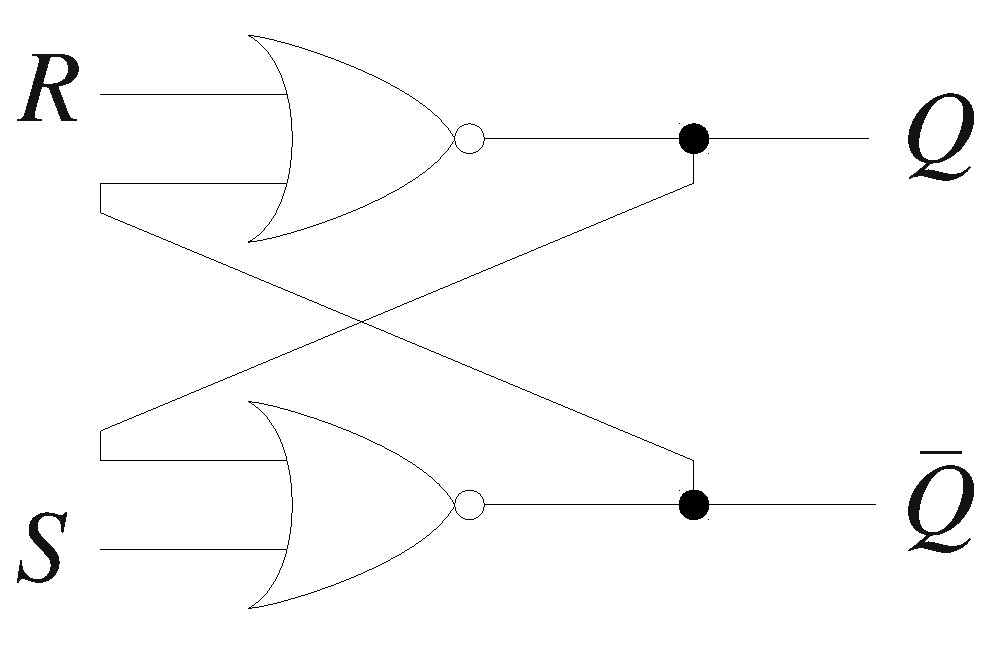
\includegraphics[width=0.30\textwidth]{include/SRlatch.pdf}
\ \ \ \ \ \ \ \ 
\begin{tikzpicture}[scale=.25]
	% STYLES
	\tikzstyle{signal} = [line width=1pt,draw=black!80]
	\tikzstyle{doublefleche} = [thin, <->, draw=violet]
	\tikzstyle{pointilles} = [thin, draw=violet, densely dotted]

	\tikzstyle{duree} = [below, pos=0.5, text=violet]

	% NOEUDS
	\node[] at (-1, 5) (S) {$S$};
	\node[] at (-1, 1) (R) {$R$};
	
	% S
	\path[signal]
		(0,6)
		-- ++ (4,0)
		-- ++ (0,-2) 
		-- ++ (12,0)
	;
	\path[doublefleche] (4, 0) -- ++(6, 0) node[duree] {$t^\downarrow$};
	\path[pointilles] (4, 4) -- ++(0, -4);

	% Q
	\path[signal]
		(0,2)
		-- ++ (10,0)
		-- ++ (0,-2) 
		-- ++ (6,0)
	;
\end{tikzpicture}

\caption{SR latch (left) and environment (right)}
\label{fig:srlatch}
\end{figure}
%-%-%-%-%-%-%-%-%-%-%-%-%-%-%-%-%-%-%-%-%-%-%-%-%-%-%-%-%-%-%

We consider a SR-latch described in, e.g., \cite{hh07}, and depicted on Fig.~\ref{fig:srlatch} left.
The possible configurations of the latch are the following ones:

\smallskip

{

\centering

\begin{tabular}{|c|c|c|c|}
	\hline
	$S$ & $R$ & $Q$ & $\overline{Q}$ \\
	\hline
	0 & 0 & latch & latch \\
	\hline
	0 & 1 & 0 & 1 \\
	\hline
	1 & 0 & 1 & 0 \\
	\hline
	1 & 1 & 0 & 0 \\
	\hline
\end{tabular}

}

\medskip

We consider an initial configuration with $R = S = 1$ and $Q = \overline{Q} = 0$.
As depicted in Fig.~\ref{fig:srlatch}, the signal~$S$ first goes down.
Then, the signal~$R$ goes down after a time~$t^\downarrow$.


We consider that the gate $\mathit{Nor}_1$ (resp. $\mathit{Nor}_2$) has a punctual parametric delay $\delta_1$ (resp. $\delta_2$).
Moreover, the parameter $t^\downarrow$ corresponds to the time duration between the fall of $S$ and the fall of $R$.


%%%%%%%%%%%%%%%%%%%%%%%%%%%%%%%%%%%%%%%%%%%%%%%%%%%%%%%%%%%%
\subsection{Parametric Reachability Analysis}
%%%%%%%%%%%%%%%%%%%%%%%%%%%%%%%%%%%%%%%%%%%%%%%%%%%%%%%%%%%%

We first perform a reachability analysis.
The launch command for \imitatordeux{} is the following one:

\code{\imitatordeuxExec{} SRlatch.imi -mode reachability}

Considering this environment, the trace set of this system is given in Fig.~\ref{fig:sr_parametric}, where the states $q_i$, $i = 0, \dots, 6$ correspond to the following values for each signal:

\smallskip

{

\centering

\begin{tabular}{|c||c|c|c|c|}
	\hline
	State & $S$ & $R$ & $Q$ & $\overline{Q}$ \\
	\hline
	$q_0$ & 1 & 1 & 0 & 0 \\
	\hline
	$q_1$ & 0 & 1 & 0 & 0 \\
	\hline
	$q_2$ & 0 & 0 & 0 & 0 \\
	\hline
	$q_3$ & 0 & 1 & 0 & 1 \\
	\hline
	$q_4$ & 0 & 0 & 0 & 1 \\
	\hline
	$q_5$ & 0 & 0 & 1 & 0 \\
	\hline
	$q_6$ & 0 & 0 & 0 & 1 \\
	\hline
\end{tabular}

}

\medskip

% %-%-%-%-%-%-%-%-%-%-%-%-%-%-%-%-%-%-%-%-%-%-%-%-%-%-%-%-%-%-%
% \begin{figure}
% \centering
% \footnotesize
% 
% \begin{tikzpicture}[scale=0.45, ->, >=stealth', auto, node distance=1.60cm, thin] % shorten >=1pt, 
%   \tikzstyle{state}=[circle, minimum size=15pt, draw=gris, text=black, inner sep=1.5pt]
% 
% 	\node[state, fill=cpale1] (Q0) at (0,3.5) {$q_0$};
% 	\node[state, fill=cpale2]         (Q1) at (4,2) {$q_1$};
% 	\node[state, fill=cpale3]         (Q2) at (4,5) {$q_2$};
% 	\node[state, fill=cpale4]         (Q3) at (8,0) {$q_3$};
% 	\node[state, fill=cpale5]         (Q4) at (8,2) {$q_4$};
% 	\node[state, fill=cpale5]         (Q5) at (8,5) {$q_5$};
% 	\node[state, fill=cpale6]         (Q6) at (8,8) {$q_6$};
% 	\node[state, fill=cpale7]         (Q7) at (12,2) {$q_7$};
% 	\node[state, fill=cpale7]         (Q8) at (12,0) {$q_8$};
% 	\node[state, fill=cpale8]         (Q9) at (12,4) {$q_9$};
% 	\node[state, fill=cpale7]        (Q10) at (12,6) {$q_{10}$};
% 	\node[state, fill=cpale8]        (Q11) at (12,8) {$q_{11}$};
% 
% 	\path
% 		(Q0) edge [double, below] node {$R^\downarrow$} (Q1)
% 		(Q0) edge [double] node {$S^\downarrow$} (Q2)
% 		(Q1) edge [double, below] node {$Q^\uparrow$} (Q3)
% 		(Q1) edge [double] node {$S^\downarrow$} (Q4)
% 		(Q2) edge [double, below] node {$R^\downarrow$} (Q5)
% 		(Q2) edge [double] node {$\overline{Q}^\uparrow$} (Q6)
% 		(Q3) edge [double] node {$S^\downarrow$} (Q8)
% 		(Q4) edge [double] node {$Q^\uparrow$} (Q7)
% 		(Q5) edge [double, below] node {$\overline{Q}^\uparrow$} (Q9)
% 		(Q5) edge [double] node {$Q^\uparrow$} (Q10)
% 		(Q6) edge [double] node {$R^\downarrow$} (Q11)
% 		;
% 
% \end{tikzpicture}
% \caption{Parametric reachability analysis of the SR latch}
% \label{fig:sr_parametric}
% \end{figure}
% %-%-%-%-%-%-%-%-%-%-%-%-%-%-%-%-%-%-%-%-%-%-%-%-%-%-%-%-%-%-%

%-%-%-%-%-%-%-%-%-%-%-%-%-%-%-%-%-%-%-%-%-%-%-%-%-%-%-%-%-%-%
\begin{figure}
\centering
\footnotesize

\begin{tikzpicture}[scale=0.45, ->, >=stealth', auto, node distance=1.60cm, thin] % shorten >=1pt, 
  \tikzstyle{state}=[circle, minimum size=15pt, draw=gris, text=black, inner sep=1.5pt]

	\node[state, fill=cpale1] (Q0) at (0,2) {$q_0$};
	\node[state, fill=cpale2]         (Q1) at (4,2) {$q_1$};
	\node[state, fill=cpale3]         (Q2) at (8,2) {$q_2$};
	\node[state, fill=cpale4]         (Q3) at (8,4) {$q_3$};
	\node[state, fill=cpale5]         (Q4) at (12,2) {$q_4$};
	\node[state, fill=cpale6]         (Q5) at (12,0) {$q_5$};
	\node[state, fill=cpale5]         (Q6) at (12,4) {$q_6$};

	\path
		(Q0) edge [double] node {$S^\downarrow$} (Q1)
		(Q1) edge [double, below] node {$R^\downarrow$} (Q2)
		(Q1) edge [double] node {$\overline{Q}^\uparrow$} (Q3)
		(Q2) edge [double] node {$\overline{Q}^\uparrow$} (Q4)
		(Q2) edge [double, below] node {$Q^\uparrow$} (Q5)
		(Q3) edge [double] node {$R^\downarrow$} (Q6)
		;

\end{tikzpicture}
\caption{Parametric reachability analysis of the SR latch}
\label{fig:sr_parametric}
\end{figure}
%-%-%-%-%-%-%-%-%-%-%-%-%-%-%-%-%-%-%-%-%-%-%-%-%-%-%-%-%-%-%

% 
% %%%%%%%%%%%%%%%%%%%%%%%%%%%%%%%%%%%%%%%%%%%%%%%%%%%%%%%%%%%%
% \subsection{Inverse Method}
% %%%%%%%%%%%%%%%%%%%%%%%%%%%%%%%%%%%%%%%%%%%%%%%%%%%%%%%%%%%%
% 
% We consider the following reference valuation $\pi_0$ of the parameters:
% 
% {\centering
% 
% \small
% 
% \begin{tabular}{r @{\ =\ } l @{\ \ \ \ \ \ } r @{\ =\ } l @{\ \ \ \ \ \ } r @{\ =\ } l @{\ \ \ \ \ \ } r @{\ =\ } l}
% $\delta_1^-$ & $1$  & $\delta_1^+$ & $4$ & $\delta_2^-$ & $2$ & $\delta_2^+$ & $5$ \\
% $T_R$ & $11$ & $T_S$ & $10$ \\
% \end{tabular}
% 
% }
% 
% Considering this environment and this reference valuation, the trace set is given in Fig.~\commentaire{to do}.
% 
% The constraint $K_0$ output by \imitatordeux{} is the following one:
% 
% \smallskip
% 
% {\centering
% 
% %  t_S_down + dNor2_u >= t_R_down + dNor1_l
% %  & dNor1_u >= dNor1_l
% %  & dNor2_u >= dNor2_l
% %  & t_S_down >= 0
% %  & t_R_down > t_S_down
% %  & t_S_down + dNor2_l > t_R_down
% %  & t_R_down + dNor1_u >= t_S_down + dNor2_l
% %  & dNor1_l >= 0
% 
% \small
% \begin{tabular}{r r @{\ } c @{\ } l @{\ \ \ \ \ } r r @{\ } c @{\ } l}
% & $T_S + \delta_2^+ $ & $ \geq $ & $ t_R + \delta_1^- $ &
% $\land$ & $T_S$ & $ \geq $ & $ 0 $ \\
% $\land$ & $T_S + \delta_2^- $ & $>$ & $T_R$ &
% $\land$ & $T_R $ & $>$ & $ T_S $ \\
% $\land$ & $T_R + \delta_1^+ $ & $ \geq $ & $ T_S + \delta_2^- $ &
% $\land$ & $\delta_1^- $ & $ \geq $ & $ 0 $\\
% \end{tabular}
% 
% }
% 
% \medskip
% 
% We checked that the trace sets under the $\pi_0$ and $K_0$ are the same.
% 

%%%%%%%%%%%%%%%%%%%%%%%%%%%%%%%%%%%%%%%%%%%%%%%%%%%%%%%%%%%%
\subsection{Behavioral Cartography Algorithm}
%%%%%%%%%%%%%%%%%%%%%%%%%%%%%%%%%%%%%%%%%%%%%%%%%%%%%%%%%%%%


Using \imitatordeux{}, we now perform a behavioral cartography of this system.
We consider the following rectangle $V_0$ for the parameters:

\smallskip

{\centering

% \small

\begin{tabular}{r @{\ $\in$ \ } l}
$ t^\downarrow $ & $[0, 10]$ \\
$ \delta_1 $ & $[0, 10]$ \\
$ \delta_2 $ & $[0, 10]$ \\
\end{tabular}

}

\smallskip

The launch command for \imitatordeux{} is the following one:

\code{\imitatordeuxExec{} SRlatch.imi SRlatch.v0 -mode cover}

We get the following six behavioral tiles.
Note that the graphical outputs, automatically generated by~\imitatordeux{} in the \code{gif} format, were rewritten in \LaTeX{} in this document.


%-%-%-%-%-%-%-%-%-%-%-%-%-%-%-%-%-%-%-%-%-%-%-%-%-%-%-%-%-%-%
\paragraph*{Tile 1.}
%-%-%-%-%-%-%-%-%-%-%-%-%-%-%-%-%-%-%-%-%-%-%-%-%-%-%-%-%-%-%
This tile corresponds to the values of the parameters verifying the following constraint:

$$ t^\downarrow = \delta_2
\ \ \land \ \ 
 \delta_1 = 0 $$

The trace set of this tile is given in Fig.~\ref{fig:sr_tile_1}.

%-%-%-%-%-%-%-%-%-%-%-%-%-%-%-%-%-%-%-%-%-%-%-%-%-%-%-%-%-%-%
\begin{figure}[ht]
\centering
\footnotesize

\begin{tikzpicture}[scale=0.45, ->, >=stealth', auto, node distance=1.60cm, thin] % shorten >=1pt, 
  \tikzstyle{state}=[circle, minimum size=15pt, draw=gris, text=black, inner sep=1.5pt]

	\node[state, fill=cpale1] (Q0) at (0,2) {$q_0$};
	\node[state, fill=cpale2]         (Q1) at (4,2) {$q_1$};
	\node[state, fill=cpale3]         (Q2) at (8,2) {$q_2$};
	\node[state, fill=cpale4]         (Q3) at (8,4) {$q_3$};
	\node[state, fill=cpale5]         (Q4) at (12,2) {$q_4$};
	\node[state, fill=cpale6]         (Q5) at (12,0) {$q_5$};
	\node[state, fill=cpale5]         (Q6) at (12,4) {$q_6$};

	\path
		(Q0) edge [double] node {$S^\downarrow$} (Q1)
		(Q1) edge [double, below] node {$R^\downarrow$} (Q2)
		(Q1) edge [double] node {$\overline{Q}^\uparrow$} (Q3)
		(Q2) edge [double] node {$\overline{Q}^\uparrow$} (Q4)
		(Q2) edge [double, below] node {$Q^\uparrow$} (Q5)
		(Q3) edge [double] node {$R^\downarrow$} (Q6)
		;

\end{tikzpicture}
\caption{Trace set of tile 1 for the SR latch}
\label{fig:sr_tile_1}
\end{figure}
%-%-%-%-%-%-%-%-%-%-%-%-%-%-%-%-%-%-%-%-%-%-%-%-%-%-%-%-%-%-%

Since $t^\downarrow = \delta_2$, $R^\downarrow$ and $\overline{Q}^\uparrow$ will occur at the same time.
Thus, the order of those two events is unspecified, which explains the choice between going to $q_2$ or $q_3$.
When in state $q_2$, either $Q^\uparrow$ can occur (since $\delta_1 = 0$), in which case the system is stable, or $\overline{Q}^\uparrow$ can occur, which also leads to stability.


%-%-%-%-%-%-%-%-%-%-%-%-%-%-%-%-%-%-%-%-%-%-%-%-%-%-%-%-%-%-%
\paragraph*{Tile 2.}
%-%-%-%-%-%-%-%-%-%-%-%-%-%-%-%-%-%-%-%-%-%-%-%-%-%-%-%-%-%-%
This tile corresponds to the values of the parameters verifying the following constraint:

$$ t^\downarrow = \delta_2
\ \ \land \ \ 
\delta_1 > 0 $$

The trace set of this tile is given in Fig.~\ref{fig:sr_tile_2}.

%-%-%-%-%-%-%-%-%-%-%-%-%-%-%-%-%-%-%-%-%-%-%-%-%-%-%-%-%-%-%
\begin{figure}[ht]
\centering
\footnotesize

\begin{tikzpicture}[scale=0.45, ->, >=stealth', auto, node distance=1.60cm, thin] % shorten >=1pt, 
  \tikzstyle{state}=[circle, minimum size=15pt, draw=gris, text=black, inner sep=1.5pt]

	\node[state, fill=cpale1] (Q0) at (0,2) {$q_0$};
	\node[state, fill=cpale2]         (Q1) at (4,2) {$q_1$};
	\node[state, fill=cpale3]         (Q2) at (8,2) {$q_2$};
	\node[state, fill=cpale4]         (Q3) at (8,4) {$q_3$};
	\node[state, fill=cpale5]         (Q4) at (12,2) {$q_4$};
% 	\node[state, fill=cpale6]         (Q5) at (12,0) {$q_5$};
	\node[state, fill=cpale5]         (Q6) at (12,4) {$q_6$};

	\path
		(Q0) edge [double] node {$S^\downarrow$} (Q1)
		(Q1) edge [double, below] node {$R^\downarrow$} (Q2)
		(Q1) edge [double] node {$\overline{Q}^\uparrow$} (Q3)
		(Q2) edge [double] node {$\overline{Q}^\uparrow$} (Q4)
% 		(Q2) edge [double, below] node {$Q^\uparrow$} (Q5)
		(Q3) edge [double] node {$R^\downarrow$} (Q6)
		;

\end{tikzpicture}
\caption{Trace set of tile 2 for the SR latch}
\label{fig:sr_tile_2}
\end{figure}
%-%-%-%-%-%-%-%-%-%-%-%-%-%-%-%-%-%-%-%-%-%-%-%-%-%-%-%-%-%-%

Since $t^\downarrow = \delta_2$, $R^\downarrow$ and $\overline{Q}^\uparrow$ will occur at the same time.
Thus, the order of those two events is unspecified, which explains the choice between going to $q_2$ or $q_3$.
When in state $q_2$, $Q^\uparrow$ can not occur (since $\delta_1 > 0$), so $\overline{Q}^\uparrow$ occurs immediately after $R^\downarrow$, which leads to stability.


%-%-%-%-%-%-%-%-%-%-%-%-%-%-%-%-%-%-%-%-%-%-%-%-%-%-%-%-%-%-%
\paragraph*{Tile 3.}
%-%-%-%-%-%-%-%-%-%-%-%-%-%-%-%-%-%-%-%-%-%-%-%-%-%-%-%-%-%-%
This tile corresponds to the values of the parameters verifying the following constraint:

$$ \delta_2 > t^\downarrow + \delta_1 $$

The trace set of this tile is given in Fig.~\ref{fig:sr_tile_3}.

%-%-%-%-%-%-%-%-%-%-%-%-%-%-%-%-%-%-%-%-%-%-%-%-%-%-%-%-%-%-%
\begin{figure}[ht]
\centering
\footnotesize

\begin{tikzpicture}[scale=0.45, ->, >=stealth', auto, node distance=1.60cm, thin] % shorten >=1pt, 
  \tikzstyle{state}=[circle, minimum size=15pt, draw=gris, text=black, inner sep=1.5pt]

	\node[state, fill=cpale1] (Q0) at (0,2) {$q_0$};
	\node[state, fill=cpale2]         (Q1) at (4,2) {$q_1$};
	\node[state, fill=cpale3]         (Q2) at (8,2) {$q_2$};
% 	\node[state, fill=cpale4]         (Q3) at (8,4) {$q_3$};
% 	\node[state, fill=cpale5]         (Q4) at (12,2) {$q_4$};
	\node[state, fill=cpale6]         (Q5) at (12,2) {$q_5$};
% 	\node[state, fill=cpale5]         (Q6) at (12,4) {$q_6$};

	\path
		(Q0) edge [double] node {$S^\downarrow$} (Q1)
		(Q1) edge [double] node {$R^\downarrow$} (Q2)
% 		(Q1) edge [double] node {$\overline{Q}^\uparrow$} (Q3)
% 		(Q2) edge [double] node {$\overline{Q}^\uparrow$} (Q4)
		(Q2) edge [double] node {$Q^\uparrow$} (Q5)
% 		(Q3) edge [double] node {$R^\downarrow$} (Q6)
		;

\end{tikzpicture}
\caption{Trace set of tile 3 for the SR latch}
\label{fig:sr_tile_3}
\end{figure}
%-%-%-%-%-%-%-%-%-%-%-%-%-%-%-%-%-%-%-%-%-%-%-%-%-%-%-%-%-%-%

In this case, since $\delta_2 > t^\downarrow + \delta_1 $, $S^\downarrow$ will occur before the gate $\mathit{Nor}_2$ has the time to change.
For the same reason, $Q^\uparrow$ will change before $\mathit{Nor}_1$ has the time to change.
With $Q = 1$, the system is now stable: $\mathit{Nor}_1$ does not change.


%-%-%-%-%-%-%-%-%-%-%-%-%-%-%-%-%-%-%-%-%-%-%-%-%-%-%-%-%-%-%
\paragraph*{Tile 4.}
%-%-%-%-%-%-%-%-%-%-%-%-%-%-%-%-%-%-%-%-%-%-%-%-%-%-%-%-%-%-%
This tile corresponds to the values of the parameters verifying the following constraint:

% t_down + dNor1 = dNor2                                                                   
%  & dNor2 >= dNor1                                                                           
%  & dNor1 > 0  

$$ t^\downarrow + \delta_1 = \delta_2 \ \ \land \ \ \delta_2 \geq \delta_1 \ \ \land \ \ \delta_1 > 0$$

The trace set of this tile is given in Fig.~\ref{fig:sr_tile_4}.

%-%-%-%-%-%-%-%-%-%-%-%-%-%-%-%-%-%-%-%-%-%-%-%-%-%-%-%-%-%-%
\begin{figure}[ht]
\centering
\footnotesize

\begin{tikzpicture}[scale=0.45, ->, >=stealth', auto, node distance=1.60cm, thin] % shorten >=1pt, 
  \tikzstyle{state}=[circle, minimum size=15pt, draw=gris, text=black, inner sep=1.5pt]

	\node[state, fill=cpale1] (Q0) at (0,2) {$q_0$};
	\node[state, fill=cpale2]         (Q1) at (4,2) {$q_1$};
	\node[state, fill=cpale3]         (Q2) at (8,2) {$q_2$};
% 	\node[state, fill=cpale4]         (Q3) at (8,4) {$q_3$};
	\node[state, fill=cpale5]         (Q4) at (12,0) {$q_4$};
	\node[state, fill=cpale6]         (Q5) at (12,2) {$q_5$};
% 	\node[state, fill=cpale5]         (Q6) at (12,4) {$q_6$};

	\path
		(Q0) edge [double] node {$S^\downarrow$} (Q1)
		(Q1) edge [double] node {$R^\downarrow$} (Q2)
% 		(Q1) edge [double] node {$\overline{Q}^\uparrow$} (Q3)
		(Q2) edge [double, below] node {$\overline{Q}^\uparrow$} (Q4)
		(Q2) edge [double] node {$Q^\uparrow$} (Q5)
% 		(Q3) edge [double] node {$R^\downarrow$} (Q6)
		;

\end{tikzpicture}
\caption{Trace set of tile 4 for the SR latch}
\label{fig:sr_tile_4}
\end{figure}
%-%-%-%-%-%-%-%-%-%-%-%-%-%-%-%-%-%-%-%-%-%-%-%-%-%-%-%-%-%-%

Since $t^\downarrow + \delta_1 = \delta_2$, both $Q^\uparrow$ or $\overline{Q}^\uparrow$ can occur.
Once one of them occured, the system gets stable, and no other change occurs.



%-%-%-%-%-%-%-%-%-%-%-%-%-%-%-%-%-%-%-%-%-%-%-%-%-%-%-%-%-%-%
\paragraph*{Tile 5.}
%-%-%-%-%-%-%-%-%-%-%-%-%-%-%-%-%-%-%-%-%-%-%-%-%-%-%-%-%-%-%
This tile corresponds to the values of the parameters verifying the following constraint:

% dNor2 > t_down
%  & t_down + dNor1 > dNor2
 
$$ \delta_2 > t^\downarrow
\ \ \land \ \ 
 t^\downarrow + \delta_1 > \delta_2 $$

The trace set of this tile is given in Fig.~\ref{fig:sr_tile_5}.

%-%-%-%-%-%-%-%-%-%-%-%-%-%-%-%-%-%-%-%-%-%-%-%-%-%-%-%-%-%-%
\begin{figure}[ht]
\centering
\footnotesize

\begin{tikzpicture}[scale=0.45, ->, >=stealth', auto, node distance=1.60cm, thin] % shorten >=1pt, 
  \tikzstyle{state}=[circle, minimum size=15pt, draw=gris, text=black, inner sep=1.5pt]

	\node[state, fill=cpale1] (Q0) at (0,2) {$q_0$};
	\node[state, fill=cpale2]         (Q1) at (4,2) {$q_1$};
	\node[state, fill=cpale3]         (Q2) at (8,2) {$q_2$};
% 	\node[state, fill=cpale4]         (Q3) at (8,4) {$q_3$};
	\node[state, fill=cpale5]         (Q4) at (12,2) {$q_4$};
% 	\node[state, fill=cpale6]         (Q5) at (12,0) {$q_5$};
% 	\node[state, fill=cpale5]         (Q6) at (12,4) {$q_6$};

	\path
		(Q0) edge [double] node {$S^\downarrow$} (Q1)
		(Q1) edge [double] node {$R^\downarrow$} (Q2)
% 		(Q1) edge [double] node {$\overline{Q}^\uparrow$} (Q3)
		(Q2) edge [double] node {$\overline{Q}^\uparrow$} (Q4)
% 		(Q2) edge [double, below] node {$Q^\uparrow$} (Q5)
% 		(Q3) edge [double] node {$R^\downarrow$} (Q6)
		;

\end{tikzpicture}
\caption{Trace set of tile 5 for the SR latch}
\label{fig:sr_tile_5}
\end{figure}
%-%-%-%-%-%-%-%-%-%-%-%-%-%-%-%-%-%-%-%-%-%-%-%-%-%-%-%-%-%-%

Since $\delta_2 > t^\downarrow$, the gate $\mathit{Nor}_2$ can not change before $R^\downarrow$ occurs.
However, since $t^\downarrow + \delta_1 > \delta_2$, the gate $\mathit{Nor}_2$ changes before $Q^\uparrow$ can occur, thus leading to event~$\overline{Q}^\uparrow$.


%-%-%-%-%-%-%-%-%-%-%-%-%-%-%-%-%-%-%-%-%-%-%-%-%-%-%-%-%-%-%
\paragraph*{Tile 6.}
%-%-%-%-%-%-%-%-%-%-%-%-%-%-%-%-%-%-%-%-%-%-%-%-%-%-%-%-%-%-%
This tile corresponds to the values of the parameters verifying the following constraint:

% t_down > dNor2
%  & dNor2 >= 0
%  & dNor1 >= 0
 
$$ t^\downarrow > \delta_2$$

The trace set of this tile is given in Fig.~\ref{fig:sr_tile_6}.

%-%-%-%-%-%-%-%-%-%-%-%-%-%-%-%-%-%-%-%-%-%-%-%-%-%-%-%-%-%-%
\begin{figure}[ht]
\centering
\footnotesize

\begin{tikzpicture}[scale=0.45, ->, >=stealth', auto, node distance=1.60cm, thin] % shorten >=1pt, 
  \tikzstyle{state}=[circle, minimum size=15pt, draw=gris, text=black, inner sep=1.5pt]

	\node[state, fill=cpale1] (Q0) at (0,2) {$q_0$};
	\node[state, fill=cpale2]         (Q1) at (4,2) {$q_1$};
% 	\node[state, fill=cpale3]         (Q2) at (8,2) {$q_2$};
	\node[state, fill=cpale4]         (Q3) at (8,2) {$q_3$};
% 	\node[state, fill=cpale5]         (Q4) at (12,2) {$q_4$};
% 	\node[state, fill=cpale6]         (Q5) at (12,0) {$q_5$};
	\node[state, fill=cpale5]         (Q6) at (12,2) {$q_6$};

	\path
		(Q0) edge [double] node {$S^\downarrow$} (Q1)
% 		(Q1) edge [double, below] node {$R^\downarrow$} (Q2)
		(Q1) edge [double] node {$\overline{Q}^\uparrow$} (Q3)
% 		(Q2) edge [double] node {$\overline{Q}^\uparrow$} (Q4)
% 		(Q2) edge [double, below] node {$Q^\uparrow$} (Q5)
		(Q3) edge [double] node {$R^\downarrow$} (Q6)
		;

\end{tikzpicture}
\caption{Trace set of tile 6 for the SR latch}
\label{fig:sr_tile_6}
\end{figure}
%-%-%-%-%-%-%-%-%-%-%-%-%-%-%-%-%-%-%-%-%-%-%-%-%-%-%-%-%-%-%

Since $t^\downarrow > \delta_2$, $\overline{Q}^\uparrow$ occurs before $S^\downarrow$.
The system is then stable.


%-%-%-%-%-%-%-%-%-%-%-%-%-%-%-%-%-%-%-%-%-%-%-%-%-%-%-%-%-%-%
\paragraph*{Cartography.}
%-%-%-%-%-%-%-%-%-%-%-%-%-%-%-%-%-%-%-%-%-%-%-%-%-%-%-%-%-%-%

We give in Fig.~\ref{fig:sr_cartography} the cartography of the SR latch example.
For the sake of simplicity of representation, we consider only parameters $\delta_1$ and $\delta_2$.
Therefore, we set $t^\downarrow = 1$.

%-%-%-%-%-%-%-%-%-%-%-%-%-%-%-%-%-%-%-%-%-%-%-%-%%
\begin{figure}[ht!]
\centering
% \scriptsize
\footnotesize

\begin{tikzpicture}[scale=.20]
	% STYLES
	\tikzstyle{axe} = [line width=1pt, ->, draw=black!80]
% 	\tikzstyle{goodzone} = [line width=2pt, draw=blue!50!black]
	\tikzstyle{v0} = [line width=1pt, draw=black, dashed]

	\tikzstyle{nomzone} = [draw=none, text=black]

	\tikzstyle{fondgris} = [fill=lightgray, draw=none]
	\tikzstyle{zone} = [draw=none]
	\tikzstyle{ligne} = [line width=2pt]

	% AXES
% 	\draw[fondgris] (0, 0) rectangle (3, 3);

	% ZONES
	% 3
	\draw[zone, fill=blue!40!white] (0, 35) -- (0, 10) -- (25, 35) -- cycle;
 	\node[nomzone] at (10, 30) {3};
	% 5
	\draw[zone, fill=green!20!white] (0, 10) -- (25, 35) -- (25, 10) -- cycle;
	\node[nomzone] at (15, 15) {5};
	% 6
	\draw[zone, fill=red!40!white] (0, 0) -- (0, 10) -- (25, 10) -- (25, 0) -- cycle;
	\node[nomzone] at (15, 5) {6};

	% AXES
	\path[axe]
		(0,0) -- ++ (27, 0);
	\path[axe]
		(0,0) -- ++ (0, 37);
	\node at (27, -2) {\large $\delta_1$};
	\node at (-2, 37) {\large $\delta_2$};
	
	% LINES
	% 4
	\draw[ligne, color=red] (0, 10) -- (25, 35);
 	\node[nomzone] at (26, 36) {4};
	% 2
	\draw[ligne, color=blue] (0, 10) -- (25, 10);
 	\node[nomzone] at (26, 10) {2};


	% POINT
	% 1
	\draw[zone, fill=green!50!black] (0,10) circle (.5);
 	\node[nomzone] at (-1, 10) {1};

	% GOOD ZONE
% 	\draw[goodzone]
% 		(8, 6) -- (8, 24) -- (9, 24) -- (27, 6) -- cycle;

	VO
	\path[v0]
		(0, 20) -- ++ (20, 0) -- ++ (0, -20) -- ++ (-20, 0) -- cycle;
	
	% VALEURS
% 	\foreach \x in {0, 1, ..., 40}
% 		\draw (0, \x) -- (-1, \x) node [left] {$\x$};
% 	\foreach \x in {0, 5, ..., 45}
% 		\draw (\x, 0) -- (\x, -1) node [below] {$\x$};
	
\end{tikzpicture}

\caption{Behavioral cartography of the SR latch according to $\delta_1$ and $\delta_2$}
\label{fig:sr_cartography}
\end{figure}
%-%-%-%-%-%-%-%-%-%-%-%-%-%-%-%-%-%-%-%-%-%-%-%-%%

Note that tile 1 corresponds to a point, and tiles 2 and 4 correspond to lines.

The rectangle $V_0$ has been represented with dashed lines.
% The number in (or next to) each tile represents the iteration number at which the corresponding constraint was computed during the algorithm run.
Note that all tiles (except tile~1) are unbounded, so that they cover, not only $V_0$, but all the positive real-valued plan.


The source code of this example is available in Appendix~\ref{app:source}.


%%%%%%%%%%%%%%%%%%%%%%%%%%%%%%%%%%%%%%%%%%%%%%%%%%%%%%%%%%%%%
%%%%%%%%%%%%%%%%%%%%%%%%%%%%%%%%%%%%%%%%%%%%%%%%%%%%%%%%%%%%%
\section{Final Remarks} \label{sec:conclusion}
%%%%%%%%%%%%%%%%%%%%%%%%%%%%%%%%%%%%%%%%%%%%%%%%%%%%%%%%%%%%%
%%%%%%%%%%%%%%%%%%%%%%%%%%%%%%%%%%%%%%%%%%%%%%%%%%%%%%%%%%%%%

The tool \imitatordeux{} allows us to solve the good parameters problem for timed automata by iterating the inverse method algorithm on the integer points of a given rectangular parameter domain~$V_0$.
In practice, our cartography algorithm covers not only (most of) $V_0$ but also a significant part of the whole parametric space beyond~$V_0$.
This is of interest to classify the behavior of the system into good or bad for dense and unbounded values of the parameters.

Our tool has been successfully applied to various examples of asynchronous circuits and protocols.

Future works include:

\begin{itemize}
	\item an automatic generation of the cartography under a graphical form (so far, only the trace sets are automatically generated under a graphical form; the cartography itself is given under the form of a list of constraints);
	\item an automatic verification of the property one wants to check, e.g., by using a tool such as \uppaal{}~\cite{lpy97};
	\item a ``dynamic'' cartography, where the scale (so far, the integers) can be refined to fill the possible holes;
	\item a backward analysis, i.e., considering a $\mathit{Pre}$ operation instead of $\mathit{Post}$ computation in Algorithm~\ref{algo:IM};
	\item the reachability analysis of a given state, and the generation of a trace from the initial state to this given state;
	\item the extension to hybrid systems;
	\item the automatic generation of the probabilities of a given property in the probabilistic framework, without the use of an external tool (e.g., \prism{}~\cite{hknp06})
	\item the automatic generation of the ``next point'' not covered by $\tiling$ without testing all the integer points (note that a random generation of points is already implemented);
	\item the possibility to compute several tiles in parallel in the cartography algorithm;
	\item a user-friendly graphical interface;
	\item the possibility to save and load sets of states.
\end{itemize}


%%%%%%%%%%%%%%%%%%%%%%%%%%%%%%%%%%%%%%%%%%%%%%%%%%%%%%%%%%%%%
\paragraph{Acknowledgments.}
%%%%%%%%%%%%%%%%%%%%%%%%%%%%%%%%%%%%%%%%%%%%%%%%%%%%%%%%%%%%%

Emmanuelle~Encrenaz and Laurent~Fribourg have been great contributors of \imitatordeux{}, on a theoretical point of view, and to find applications both from the literature and real case studies.
Abdelrezzak~Bara provided several examples from the hardware literature.
Jeremy~Sproston provided examples from the probabilistic community.
Bertrand~Jeannet has been of great help on the installation part, and the linking with Apron~\cite{jm09}.
Ulrich~K\"uhne started to improve \imitatordeux{}, and added the link with PPL.



%%%%%%%%%%%%%%%%%%%%%%%%%%%%%%%%%%%%%%%%%%%%%%%%%%%%%%%%%%%%%
%%%%%%%%%%%%%%%%%%%%%%%%%%%%%%%%%%%%%%%%%%%%%%%%%%%%%%%%%%%%%
\bibliographystyle{plain}
\bibliography{biblio}
%%%%%%%%%%%%%%%%%%%%%%%%%%%%%%%%%%%%%%%%%%%%%%%%%%%%%%%%%%%%%
%%%%%%%%%%%%%%%%%%%%%%%%%%%%%%%%%%%%%%%%%%%%%%%%%%%%%%%%%%%%%

\newpage

\appendix

%%%%%%%%%%%%%%%%%%%%%%%%%%%%%%%%%%%%%%%%%%%%%%%%%%%%%%%%%%%%%
%%%%%%%%%%%%%%%%%%%%%%%%%%%%%%%%%%%%%%%%%%%%%%%%%%%%%%%%%%%%%
\section{Source Code of the Example} \label{app:source}
%%%%%%%%%%%%%%%%%%%%%%%%%%%%%%%%%%%%%%%%%%%%%%%%%%%%%%%%%%%%%
%%%%%%%%%%%%%%%%%%%%%%%%%%%%%%%%%%%%%%%%%%%%%%%%%%%%%%%%%%%%%

%%%%%%%%%%%%%%%%%%%%%%%%%%%%%%%%%%%%%%%%%%%%%%%%%%%%%%%%%%%%%
\subsection{Main Input File}
%%%%%%%%%%%%%%%%%%%%%%%%%%%%%%%%%%%%%%%%%%%%%%%%%%%%%%%%%%%%%

\FichierImitator{include/SRlatch.imi}



%%%%%%%%%%%%%%%%%%%%%%%%%%%%%%%%%%%%%%%%%%%%%%%%%%%%%%%%%%%%%
\subsection{$V_0$ File}
%%%%%%%%%%%%%%%%%%%%%%%%%%%%%%%%%%%%%%%%%%%%%%%%%%%%%%%%%%%%%

\FichierImitator{include/SRlatch.v0}



\newpage

%%%%%%%%%%%%%%%%%%%%%%%%%%%%%%%%%%%%%%%%%%%%%%%%%%%%%%%%%%%%%
%%%%%%%%%%%%%%%%%%%%%%%%%%%%%%%%%%%%%%%%%%%%%%%%%%%%%%%%%%%%%
\section{Complete Grammar} \label{app:grammar}
%%%%%%%%%%%%%%%%%%%%%%%%%%%%%%%%%%%%%%%%%%%%%%%%%%%%%%%%%%%%%
%%%%%%%%%%%%%%%%%%%%%%%%%%%%%%%%%%%%%%%%%%%%%%%%%%%%%%%%%%%%%


%%%%%%%%%%%%%%%%%%%%%%%%%%%%%%%%%%%%%%%%%%%%%%%%%%%%%%%%%%%%%
\subsection{Grammar of the Input File}
%%%%%%%%%%%%%%%%%%%%%%%%%%%%%%%%%%%%%%%%%%%%%%%%%%%%%%%%%%%%%

\imitatordeux{} input is described by the following grammar.
Non-terminals appear within angled parentheses.
A non-terminal followed by two colons is defined by the list of immediately following non-blank lines, each of which represents a legal expansion.
Input characters of terminals appear in typewritter font.
The meta symbol \emptystring{} denotes the empty string.

The text \npec{in green} is not taken into account by \imitatordeux{}, but is allowed (or sometimes necessary) in order to allow the compatibility with \hytech{} files.


%------------------------------------------------------------
\regleGrammaire{imitator\_input}
%------------------------------------------------------------
\begin{tabular}{l l}
	\  & \nt{automata\_descriptions} \nt{init} \\
\end{tabular}

\medskip


We define each of those two components below.

%-%-%-%-%-%-%-%-%-%-%-%-%-%-%-%-%-%-%-%-%-%-%-%-%-%-%-%-%-%-%
\subsubsection{Automata Descriptions}
%-%-%-%-%-%-%-%-%-%-%-%-%-%-%-%-%-%-%-%-%-%-%-%-%-%-%-%-%-%-%

%------------------------------------------------------------
\regleGrammaire{automata\_descriptions}
%------------------------------------------------------------
\begin{tabular}{l l}
	\  & \nt{declarations} \nt{automata} \\
\end{tabular}

%------------------------------------------------------------
\regleGrammaire{declarations}
%------------------------------------------------------------
\begin{tabular}{l l}
	\  & \code{var} \nt{var\_lists} \\
\end{tabular}

%------------------------------------------------------------
\regleGrammaire{var\_lists}
%------------------------------------------------------------
\begin{tabular}{l l}
	\  & \nt{var\_list} \code{:} \nt{var\_type} \code{;} \nt{var\_lists} \\
	$|$ & \emptystring
\end{tabular}

%------------------------------------------------------------
\regleGrammaire{var\_list}
%------------------------------------------------------------
\begin{tabular}{l l}
	\  & \code{<name>} \\
	$|$ & \code{<name>} \code{,} \nt{var\_list}
\end{tabular}

%------------------------------------------------------------
\regleGrammaire{var\_type}
%------------------------------------------------------------
\begin{tabular}{l l}
	\  & \code{clock} \\
	$|$ & \code{discrete} \\
	$|$ & \code{parameter} \\
\end{tabular}

%------------------------------------------------------------
\regleGrammaire{automata}
%------------------------------------------------------------
\begin{tabular}{l l}
	\  & \nt{automaton} \nt{automata} \\
	$|$ & \emptystring \\
\end{tabular}

%------------------------------------------------------------
\regleGrammaire{automaton}
%------------------------------------------------------------
\begin{tabular}{l l}
	\  & \code{automaton} \code{<name>} \nt{prolog} \nt{locations} \code{end} \\
\end{tabular}

%------------------------------------------------------------
\regleGrammaire{prolog}
%------------------------------------------------------------
\begin{tabular}{l l}
	\  & \npec{\nt{initialization}} \nt{sync\_labels} \\
	$|$ & \nt{sync\_labels} \npec{\nt{initialization}} \\
	$|$ & \nt{sync\_labels} \\
\end{tabular}

%------------------------------------------------------------
\regleGrammaire{initialization}
%------------------------------------------------------------
\npec{
\begin{tabular}{l l}
	\  & \code{initially} \code{<name>} \nt{state\_initialization} \code{;} \\
\end{tabular}
}

%------------------------------------------------------------
\regleGrammaire{state\_initialization}
%------------------------------------------------------------
\npec{
\begin{tabular}{l l}
	\  & \code{\&} \nt{convex\_predicate} \\
	$|$ & \emptystring \\
\end{tabular}
}

%------------------------------------------------------------
\regleGrammaire{prolog}
%------------------------------------------------------------
\begin{tabular}{l l}
	\  & \code{synclabs} \code{:} \nt{sync\_var\_list} \code{;} \\
\end{tabular}

%------------------------------------------------------------
\regleGrammaire{sync\_var\_list}
%------------------------------------------------------------
\begin{tabular}{l l}
	\  & \nt{sync\_var\_nonempty\_list} \\
	$|$ & \emptystring \\
\end{tabular}

%------------------------------------------------------------
\regleGrammaire{sync\_var\_nonempty\_list}
%------------------------------------------------------------
\begin{tabular}{l l}
	\  & \code{<name>} \code{,} \nt{sync\_var\_nonempty\_list} \\
	$|$ & \code{<name>} \\
\end{tabular}

%------------------------------------------------------------
\regleGrammaire{locations}
%------------------------------------------------------------
\begin{tabular}{l l}
	\  & \nt{location} \nt{locations} \\
	$|$ & \emptystring \\
\end{tabular}

%------------------------------------------------------------
\regleGrammaire{locations}
%------------------------------------------------------------
\begin{tabular}{l l}
	\  & \code{loc} \code{<name>} \code{:} \code{while} \nt{convex\_predicate} \code{wait} \npec{\code{()}} \nt{transitions} \\
	$|$ & \code{loc} \code{<name>} \code{:} \code{while} \nt{convex\_predicate} \code{wait} \nt{transitions} \\
\end{tabular}

%------------------------------------------------------------
\regleGrammaire{transitions}
%------------------------------------------------------------
\begin{tabular}{l l}
	\  & \nt{transition} \nt{transitions} \\
	$|$ & \emptystring \\
\end{tabular}

%------------------------------------------------------------
\regleGrammaire{transition}
%------------------------------------------------------------
\begin{tabular}{l l}
	\  & \code{when} \nt{convex\_predicate} \nt{update\_synchronization} \code{goto} \code{<name>} \code{;} \\
\end{tabular}

%------------------------------------------------------------
\regleGrammaire{update\_synchronization}
%------------------------------------------------------------
\begin{tabular}{l l}
	\  & \nt{updates} \\
	$|$ & \nt{syn\_label} \\
	$|$ & \nt{updates} \nt{syn\_label} \\
	$|$ & \nt{syn\_label} \nt{updates} \\
	$|$ & \emptystring \\
\end{tabular}

%------------------------------------------------------------
\regleGrammaire{updates}
%------------------------------------------------------------
\begin{tabular}{l l}
	\  & \code{do} \code{(} \nt{update\_list} \code{)} \\
\end{tabular}

%------------------------------------------------------------
\regleGrammaire{update\_list}
%------------------------------------------------------------
\begin{tabular}{l l}
	\  & \nt{update\_nonempty\_list} \\
	$|$ & \emptystring \\
\end{tabular}

%------------------------------------------------------------
\regleGrammaire{update\_nonempty\_list}
%------------------------------------------------------------
\begin{tabular}{l l}
	\  & \nt{update} \code{,} \nt{update\_nonempty\_list} \\
	$|$ & \nt{update} \\
\end{tabular}

%------------------------------------------------------------
\regleGrammaire{update\_nonempty\_list}
%------------------------------------------------------------
\begin{tabular}{l l}
	\  & \code{<name>} \code{'} \code{=} \nt{linear\_expression} \\
\end{tabular}

%------------------------------------------------------------
\regleGrammaire{syn\_label}
%------------------------------------------------------------
\begin{tabular}{l l}
	\  & \code{sync} \code{<name>} \\
\end{tabular}



%------------------------------------------------------------
\regleGrammaire{convex\_predicate}
%------------------------------------------------------------
\begin{tabular}{l l}
	\  & \nt{linear\_constraint} \code{\&} \nt{convex\_predicate} \\
	$|$ & \nt{linear\_constraint} \\
\end{tabular}

%------------------------------------------------------------
\regleGrammaire{linear\_constraint}
%------------------------------------------------------------
\begin{tabular}{l l}
	\  & \nt{linear\_expression} \nt{relop} \nt{linear\_expression} \\
	$|$ & \code{True} \\
	$|$ & \code{False} \\
\end{tabular}

%------------------------------------------------------------
\regleGrammaire{relop}
%------------------------------------------------------------
\begin{tabular}{l l}
	\  & \code{<} \\
	$|$ & \code{<=} \\
	$|$ & \code{=} \\
	$|$ & \code{>=} \\
	$|$ & \code{>} \\
\end{tabular}

%------------------------------------------------------------
\regleGrammaire{linear\_expression}
%------------------------------------------------------------
\begin{tabular}{l l}
	\  & \nt{linear\_term} \\
	$|$ & \nt{linear\_expression} \code{+} \nt{linear\_term} \\
	$|$ & \nt{linear\_expression} \code{-} \nt{linear\_term} \\
\end{tabular}

%------------------------------------------------------------
\regleGrammaire{linear\_term}
%------------------------------------------------------------
\begin{tabular}{l l}
	\  & \nt{rational} \\
	$|$ & \nt{rational} \code{<name>} \\
	$|$ & \nt{rational} \code{*} \code{<name>} \\
	$|$ & \code{<name>} \\
	$|$ & \code{(} \nt{linear\_term} \code{)} \\
\end{tabular}

%------------------------------------------------------------
\regleGrammaire{rational}
%------------------------------------------------------------
\begin{tabular}{l l}
	\  & \nt{integer} \\
	$|$ & \nt{integer} \code{/} \nt{pos\_integer}  \\
\end{tabular}

%------------------------------------------------------------
\regleGrammaire{integer}
%------------------------------------------------------------
\begin{tabular}{l l}
	\  & \nt{pos\_integer} \\
	$|$ & \code{-} \nt{pos\_integer}  \\
\end{tabular}

%------------------------------------------------------------
\regleGrammaire{pos\_integer}
%------------------------------------------------------------
\begin{tabular}{l l}
	\  & \code{<int>} \\
\end{tabular}




%-%-%-%-%-%-%-%-%-%-%-%-%-%-%-%-%-%-%-%-%-%-%-%-%-%-%-%-%-%-%
\subsubsection{Initial State}
%-%-%-%-%-%-%-%-%-%-%-%-%-%-%-%-%-%-%-%-%-%-%-%-%-%-%-%-%-%-%

%------------------------------------------------------------
\regleGrammaire{init}
%------------------------------------------------------------
\begin{tabular}{l l}
	\  & \npec{\nt{init\_declaration}} \nt{init\_definition} \npec{\nt{reach\_command}} \\
\end{tabular}

%------------------------------------------------------------
\regleGrammaire{init\_declaration}
%------------------------------------------------------------
\begin{tabular}{l l}
	\  & \npec{\code{var} \code{init} \code{:} \code{region} \code{;}} \\
	$|$ & \emptystring \\
\end{tabular}

%------------------------------------------------------------
\regleGrammaire{reach\_command}
%------------------------------------------------------------
\begin{tabular}{l l}
	\  & \npec{\code{print} \code{(} \code{reach} \code{forward} \code{from} \code{init} \code{endreach} \code{)} \code{;}} \\
	$|$ & \emptystring \\
\end{tabular}

%------------------------------------------------------------
\regleGrammaire{init\_definition}
%------------------------------------------------------------
\begin{tabular}{l l}
	\  & \code{init} \code{:=} \nt{region\_expression} \code{;} \\
\end{tabular}

%------------------------------------------------------------
\regleGrammaire{region\_expression}
%------------------------------------------------------------
\begin{tabular}{l l}
	\  & \nt{state\_predicate} \\
	$|$ & \code{(} \nt{region\_expression} \code{)} \\
	$|$ & \nt{region\_expression} \code{\&} \nt{region\_expression} \\
\end{tabular}

%------------------------------------------------------------
\regleGrammaire{state\_predicate}
%------------------------------------------------------------
\begin{tabular}{l l}
	\  & \code{loc} \code{[} \code{<name>} \code{]} \code{=} \code{<name>} \\
	$|$ & \nt{linear\_constraint} \\
\end{tabular}



%%%%%%%%%%%%%%%%%%%%%%%%%%%%%%%%%%%%%%%%%%%%%%%%%%%%%%%%%%%%%
% \subsection{Grammar of reference valuation file}
%%%%%%%%%%%%%%%%%%%%%%%%%%%%%%%%%%%%%%%%%%%%%%%%%%%%%%%%%%%%%
% TO DO 

%%%%%%%%%%%%%%%%%%%%%%%%%%%%%%%%%%%%%%%%%%%%%%%%%%%%%%%%%%%%%
% \subsection{Grammar of reference rectangle file}
%%%%%%%%%%%%%%%%%%%%%%%%%%%%%%%%%%%%%%%%%%%%%%%%%%%%%%%%%%%%%
% TO DO 


%%%%%%%%%%%%%%%%%%%%%%%%%%%%%%%%%%%%%%%%%%%%%%%%%%%%%%%%%%%%%
\subsection{Reserved Words}
%%%%%%%%%%%%%%%%%%%%%%%%%%%%%%%%%%%%%%%%%%%%%%%%%%%%%%%%%%%%%

The following words are keywords and cannot be used as names for automata, variables, synchronization labels or locations. 

\code{and},
\code{automaton},
\code{clock},
\code{discrete},
\code{do},
\code{end},
\code{endreach},
\code{False},
\code{forward},
\code{from},
\code{goto},
\code{if},
\code{in},
\code{init},
\code{initially},
\code{loc},
\code{locations},
\code{not},
\code{or},
\code{parameter},
\code{print},
\code{reach},
\code{region},
\code{sync},
\code{synclabs},
\code{True},
\code{var},
\code{wait},
\code{when},
\code{while}

\end{document}

